\documentclass[a4paper,11pt]{report}


%%%%%%%%%%%%%%%%%%%%%%%%%%%%
% University of Sussex thesis template
%%%%%%%%%%%%%%%%%%%%%%%%%%%%
% Modification History
%
% Based on usthesis.cls by Jonathon Read
% http://www.cogs.susx.ac.uk/users/jlr24/latex.html
% Modified by Anthony Smith, Feb 2007
% Incorporated into single thesis.tex file, Anthony Smith, 30 June 2008
% Minor alterations to page numbering, AJS, 25 July 2008
% New alternative hyperref options for print version, AJS, 11 Sep 2008
% "DRAFT" on header, AJS, 12 Sep 2008
%%%%%%%%%%%%%%%%%%%%%%%%%%%%


%%%%%%%%%%%%%%%%%%%%%%%%%%%%
% LINE SPACING
\newcommand{\linespacing}{1.5}
\renewcommand{\baselinestretch}{\linespacing}
%%%%%%%%%%%%%%%%%%%%%%%%%%%%


%%%%%%%%%%%%%%%%%%%%%%%%%%%%
% BIBLIOGRAPHY STYLE
% \usepackage{natbib}
% \bibliographystyle{plain} for [1], [2] etc.
% \bibliographystyle{apalike}
%%%%%%%%%%%%%%%%%%%%%%%%%%%%


%%%%%%%%%%%%%%%%%%%%%%%%%%%%
% OTHER FORMATTING/LAYOUT DECLARATIONS
% Graphics
\usepackage{graphicx,color}
\usepackage{epstopdf}
\usepackage[brazil]{babel}
\usepackage[T1]{fontenc}
\usepackage{ae} 
\usepackage[ansinew]{inputenc} 
% Some packages used in my master's thesis
\usepackage{indentfirst}
% The left-hand-side should be 40mm.  The top and bottom margins should be
% 25mm deep.  The right hand margin should be 20mm.
\usepackage[a4paper,top=2.5cm,bottom=2.5cm,left=3cm,right=3cm,headsep=10pt]{geometry}
\flushbottom
% Pages should be numbered consecutively thorugh the main text.  Page numbers
% should be located centrally at the top of the page.
\usepackage{fancyhdr}
%\fancypagestyle{plain}{
	% \fancyhf{}
	% Add "DRAFT: <today's date>" to header (comment out the following to remove)
	% \lhead{\textit{DRAFT: \today}}
	%
	% \chead{\thepage}
	% \renewcommand{\headrulewidth}{0pt}
%}
\pagestyle{plain}
%%%%%%%%%%%%%%%%%%%%%%%%%%%%


%%%%%%%%%%%%%%%%%%%%%%%%%%%%
% ANY OTHER DECLARATIONS HERE:

%%%%%%%%%%%%%%%%%%%%%%%%%%%%


%%%%%%%%%%%%%%%%%%%%%%%%%%%%
% HYPERREF
\usepackage[colorlinks,pdfusetitle,urlcolor=blue,citecolor=blue,linkcolor=blue,bookmarksnumbered,plainpages=false]{hyperref}
% For print version, use this instead:
%\usepackage[pdfusetitle,bookmarksnumbered,plainpages=false]{hyperref}
%\usepackage{backref}
%\renewcommand{\backrefpagesname}{Cited on}
%%%%%%%%%%%%%%%%%%%%%%%%%%%%


%%%%%%%%%%%%%%%%%%%%%%%%%%%%
% BEGIN DOCUMENT
\begin{document}
%%%%%%%%%%%%%%%%%%%%%%%%%%%%


%%%%%%%%%%%%%%%%%%%%%%%%%%%%
% PREAMBLE: roman page numbering i, ii, iii, ...
\pagenumbering{roman}
%%%%%%%%%%%%%%%%%%%%%%%%%%%%


%%%%%%%%%%%%%%%%%%%%%%%%%%%%
%% TITLE PAGE: The title page should give the following information:
%%	(i) the full title of the thesis and the sub-title if any;
%%	(ii) the full name of the author;
%%	(iii) the qualification aimed for;
%%	(iv) the name of the University of Sussex;
%%	(v) the month and year of submission.
\thispagestyle{empty}
\begin{flushright}

\includegraphics[width=3cm]{puclogo}
\end{flushright}	
\vskip40mm
\begin{center}
% TITLE FENOMENOS DE PROPAGACAO EM REDES COMPLEXAS?

\huge\textbf{Exame de Qualifica\c{c}\~ao}
\vskip2mm
% SUBTITLE (optional)
\LARGE\textit{Fen\^omenos de Propaga\c{c}\~ao em Redes Complexas}
\vskip5mm
% AUTHOR
\Large\textbf{Aluno: Marlon Ramos}\\
\Large\textbf{Orientadora: Celia Anteneodo}
\normalsize
\end{center}
\vfill
\begin{flushleft}
\large
% QUALIFICATION
Departamento de F\'isica\\
Pontif\'icia Universidade Cat\'olica do Rio de Janeiro\\
% DATE OF SUBMISSION
Junho 2012
\end{flushleft}		
%%%%%%%%%%%%%%%%%%%%%%%%%%%%


%%%%%%%%%%%%%%%%%%%%%%%%%%%%
% SUMMARY PAGE
\thispagestyle{empty}
\newpage
\null\vskip10mm
\begin{center}
\large
\underline{Pontif\'icia Universidade Cat\'olica do Rio de Janeiro}
\vskip20mm
% AUTHOR, QUALIFICATION
\textsc{Marlon Ramos}
\vskip20mm
% TITLE
\underline{\textsc{Exame de Qualifica\c{c}\~ao}}
\vskip0mm
% SUBTITLE (optional)
\underline{\textsc{Fen\^omenos de Propaga\c{c}\~ao em Redes Complexas}}
\vskip20mm
\underline{\textsc{Resumo}}
\vskip2mm
\end{center}
% Change line spacing
\renewcommand{\baselinestretch}{1.0}
\small\normalsize
% SUMMARY HERE (300 word limit for most subjects):

%%%%%%%%%%%%%%%%%%%%%%%%%%%%


%%%%%%%%%%%%%%%%%%%%%%%%%%%%
% ACKNOWLEDGEMENTS
% \chapter*{Agradecimentos}
% \renewcommand{\baselinestretch}{\linespacing}
% \small\normalsize
% ACKNOWLEDGEMENTS HERE:

%%%%%%%%%%%%%%%%%%%%%%%%%%%%


%%%%%%%%%%%%%%%%%%%%%%%%%%%%
% TABLE OF CONTENTS, LISTS OF TABLES & FIGURES
\newpage
\pdfbookmark[0]{Contents}{contents_bookmark}
\tableofcontents
%\listoftables
%\phantomsection
%\addcontentsline{toc}{chapter}{List of Tables}
%\listoffigures
%\phantomsection
%\addcontentsline{toc}{chapter}{List of Figures}
%%%%%%%%%%%%%%%%%%%%%%%%%%%%


%%%%%%%%%%%%%%%%%%%%%%%%%%%%
% MAIN THESIS TEXT: arabic page numbering 1, 2, 3, ...
\newpage
\pagenumbering{arabic}
%%%%%%%%%%%%%%%%%%%%%%%%%%%%


%-----------------------------------------------------
% Chapter: Introducao e Metologia
%-----------------------------------------------------


\chapter{Introdu\c{c}\~ao e Metodologia}
\label{chap:intro}

\section{Introdu\c{c}\~ao e Motiva\c{c}\~ao}

CONTAGIO: (biologia e sociologia)  keywords PRx rumor+spreading

O foco do trabalho \'e o estudo de fen\^omenos de espalhamento em redes sociais. 



FOCO: fenomenos de propagacao em meios sociais: 

-difusao de rumores, informacoes

-surgimento de consenso na adopcao de inovacoes tecnologicas, 
 formacao de opinioes, da linguagem, diseminacao de ideias, 
da corrupcao, praticas sociais, etc.

-epidemias de doencas infecciosas 

diversos fenomenos governados por interacoes sociais
que podem evoluir para estados finais fragmentados desordenados 
ou de consenso, em que todos os individuos sao atingidos por 
informacoes ou doencas (consenso de opinioes, epidemias, 
respectivamente) ou adoptam um mesmo padrao comportamental 
(opiniao, linguagem) \cite{BOCCALETTI:2006gb}

a pergunta fundamental eh como esses estados estacionarios emergem, 
quais os mecanismos e como exercer controle sobre os mesmos


a topologia da rede em que as interacoes ocorrem tambem eh 
crucial para determinar as propriedades emergentes 

\section{Metologia} 

analogia com problemas de fisica estatistica, tr. de fase, percolacao, difusao, etc

fisica est: analogia com sistemas fisicos (magneticos tipo Ising, 1/2 ou 1)

uso de redes complexas

%-----------------------------------------------------
% Chapter: Modelos
%-----------------------------------------------------
\chapter{Revis\~ao Bibliogr\'afica}
\label{chap:models}

\section{Modelos}

Uma das maiores motiva\c{c}\~oes para o estudo de redes sociais \'e o seu papel no espalhamento de doen\c{c}as. Doen\c{c}as se espalham atrav\'es da rede de contatos entre indiv\'iduos, por exemplo: doen\c{c}as respirat\'orias se espalham quando pessoas que est\~ao no mesmo ambiente e respiram o mesmo ar, certas doen\c{c}as se transmitem quando as pessoas se tocam, etc. O padr\~ao de contatos entre as pessoas pode ser representado como uma rede e por isso o enfor\c{c}o para se caracterizar bem a estrutura das redes sociais. Um t\'opico relacionado \'e o espalhamento de v\'irus de computador e o espalhamento de rumores e not\'icias.    
Nesse trabalho, vamos descrever os modelos cl\'assicos de epidemias e espalhamento de rumores. 

A biologia do que acontece dentro de uma pessoa quando ela \'e infectada com uma doen\c{c}a \'e complicada. H\'a uma luta do pat\^ogeno com o sistema imunol\'ogico, o que pode levar a cura, uma infec\c{c}\~ao permanente ou a morte. Para estudar o espalhamento de uma doen\c{c}a ter\'iamos que levar tudo isso em conta, o que n\~ao \'e poss\'ivel na pr\'atica. 

Na formula\c{c}\~ao matemt\'atica usual de uma epidemia a din\^amica da doen\c{c}a \'e reduzida \`a mudan\c{c}a entre alguns estados. Na vers\~ao mais simples de todas, trabalhamos com dois estados somente: suscept\'iveis e infectados. Um indiv\'iduo no estado suscept\'ivel n\~ao tem a doen\c{c}a mas pode vir a ser infectado. O individuo no estado infectado \'e aquele que tem a doen\c{c}a e pode transmiti-la caso tenha contato com um algu\'em susceptivel. Essa \'e uma simplifica\c{c}\~ao forte, mas captura as caracter\'isticas b\'asicas da doen\c{c}a e \'e \'util quando queremos saber o que acontece com uma dada popula\c{c}\~ao e n\~ao o que acontece com cada um dos membros da popula\c{c}\~ao. 

A abordagem usual n\~ao leva em conta a estrutura da rede de contatos. Fazemos uso de uma aproxima\c{c}\~ao chamada homogeneous mixing hypothesis em que supomos que cada um dos indiv\'iduos tem a mesma probabilidade, por unidade de tempo, de entrar em contato com qualquer outro. As pessoas se encontram completamente ao acaso nessa abordagem. \'E claro que essa n\~ao \'e uma hip\'otese real\'istica porque as pessoas tem contato direto com uma fra\c{c}\~ao pequena da popula\c{c}\~ao e esses contatos n\~ao s\~ao ao acaso. Exatamente por isso o estudo de redes \'e importante. 


Consideremos uma doen\c{c}a que se espalha em uma dada popula\c{c}\~ao. Vamos denotar por $S(t)$ e $I(t)$ o n\'umero de individuos suscept\'iveis e infectados no tempo $t$ respectivamente. O n\'umero de infectados aumenta quando indiv\'iduos suscept\'iveis entram em contato com infectados. Suponha que as pessoas se encontram ao acaso, e fa\c{c}am contato por um tempo suficiente para que haja cont\'agio, com uma taxa $\beta$, \textit{i. e.} cada membro da popula\c{c}\~ao faz em m\'edia $\beta$ contatos com outras pessoas escolhidas ao acaso por unidade de tempo. 

Um cont\'agio acontece s\'o quando um membro suscept\'ivel da popula\c{c}\~ao se encontra com um infectado. Se o n\'umero total de pessoas \'e $n$, a probabilidade de encontrar uma pessoa suscept\'ivel ao acaso \'e $S/n$. Da\'i, cada infectado encontra em m\'edia $\beta S/n$ indiv\'iduos suscept\'iveis por unidade de tempo. Como temos $I$ pessoas infectadas, a taxa de novas infe\c{c}\~oes \'e $\beta SI/n$ e ficamos com a seguinte equa\c{c}\~ao diferencial para o n\'umero de infectados:

\begin{equation}
\frac{dI}{dt}=\beta SI/n.
\label{eq:inf-SI}
\end{equation}

O n\'umero de suscept\'iveis decresce com a mesma taxa

\begin{equation}
\frac{dS}{dt}=-\beta SI/n
\label{eq:suc-SI}
\end{equation}

Esse \'e o modelo conhecido como \textit{fully mixed susceptible-infected model} ou SI. \'E mais comum trabalhar com fra\c{c}\~oes de indiv\'iduos, vamos definir novas vari\'aveis $s=S/n$ e $i=I/n$, com isso as equa\c{c}\~oes \ref{eq:inf-SI} e \ref{eq:suc-SI} ficam na forma:

\begin{equation}
\frac{di}{dt}=\beta si.
\label{eq:inf-SI-den}
\end{equation}

\begin{equation}
\frac{ds}{dt}=-\beta si
\label{eq:suc-SI-den}
\end{equation}

Nesse modelo a popula\c{c}\~ao \'e constante, ent\~ao, na verdade podemos reduzir as equa\c{c}\~oes \ref{eq:inf-SI-den} e \ref{eq:suc-SI-den} \`a uma \'unica atrav\'es da rela\c{c}\~ao $s+i=1$, o que nos d\'a

\begin{equation}
\frac{di}{dt}=\beta i(i-1).
\label{eq:log-eq}
\end{equation}

Essa equa\c{c}\~ao \'e a conhecida equa\c{c}\~ao log\'istica que aparece em muitas outras situa\c{c}\~oes e tem como solu\c{c}\~ao

\begin{equation}
i(t)=\frac{i_0 e^{\beta t}}{1-i_0+i_0 e^{\beta t}},
\label{eq:log-sol}
\end{equation}
onde $i_0=i(0)$. A express\~ao acima tem a forma mostrada em \ref{fig:logistic}. Ela cresce exponencialmente para tempos curtos, o que corresponde a fase inicial da doen\c{c}a onde h\'a muitos indiv\'iduos suscept\'iveis, mas satura eventualmente, a medida em que a epidemia avan\c{c}a e fica mais dif\'icil encontrar novas v\'itimas. 

\begin{figure}[ht!]
\begin{center}
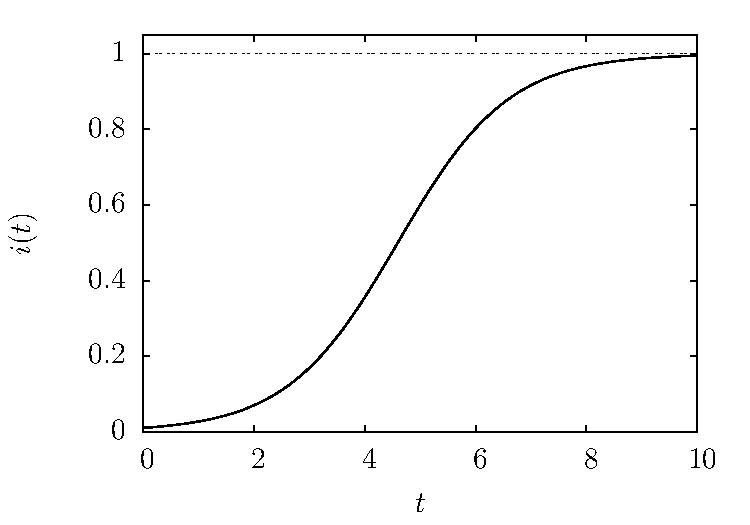
\includegraphics[scale=0.8]{./images/logistic.pdf}
\label{fig:logistic}
\caption{Curva cl\'assica da equa\c{c}\~ao log\'istica. Usei $i_0=1\%$.}
\end{center}
\end{figure}


\section{Modelo SIR}  

No modelo SI, uma vez que a pessoa seja infectada, ela permanece nesse estado para sempre, mas em muitas doen\c{c}as as pessoas conseguem se recuperar da infec{c}\~ao depois de um tempo e uma vez recuperadas adquirem imunidade. Essa observa\c{c}\~ao motiva a introdu\c{c}\~ao de um novo estado: os recuperados $R$. Em outras doen\c{c}as, as pessoas n\~ao se recuperam, pelo contr\'ario, elas morrem. Do ponto de vista do indiv\'iduo isso \'e exatamente o contr\'ario de ficar curado, mas para a doen\c{c}a tanto faz uma pessoa estar morta ou imune, de qualquer maneira o n\'umero de  hospedeiros potenciais \'e reduzido. Por isso, a letra $R$ algumas significa removidos. Nesse modelo, as duas situa\c{c}\~oes s\~ao equivalentes. O acr\^onimo SIR signica \textit{susceptible-infected-removed}.

O modelo tem duas etapas. Primeiro, uma pessoa se infecta quando entra em contato com algu\'em que tem a doen\c{c}a, os contatos ocorrem com a mesma taxa $\beta$ do modelo SI. Na outra etapa, as pessoas infectadas se recuperam (ou morrem) com uma taxa $\gamma$. Em termos das densidades $s$, $i$ e $r$, o modelo SIR tem as equa\c{c}\~oes:

\begin{equation}
\frac{ds}{dt}=-\beta si,
\label{eq:suc-SIR-den}
\end{equation}

\begin{equation}
\frac{di}{dt}=\beta si-\gamma i,
\label{eq:inf-SIR-den}
\end{equation}

\begin{equation}
\frac{dr}{dt}=\gamma i,
\label{eq:rem-SIR-den}
\end{equation}
e completamos a formula\c{c}\~ao com as condi\c{c}\~oes iniciais

\begin{equation}
s(0)=s_0>0, \quad i(0)=i_0>0, \quad r(0)=0.
\end{equation}

Temos tamb\'em a equa\c{c}\~ao de conserva\c{c}\~ao $s+r+i=1$, que \'e automaticamente satisfeita pelas equa\c{c}\~oes acima. 

A primeira quest\~ao relevante a ser respondida \'e se existir\'a uma epidemia ou n\~ao e, se houver, como ser\'a a evolu\c{c}\~ao temporal.

Pela equa\c{c}\~ao \ref{eq:inf-SIR-den}, temos para $t=0$

\begin{equation}
\frac{di}{dt}\Bigg|_{t=0}=i_0(\beta s_0-\gamma)\ge 0\quad \mbox{se}\quad s_0\ge \frac{\gamma}{\beta}\equiv \rho 
\end{equation}

Dado que $ds/dt<0$, ent\~ao temos que $s<s_0$ sempre, portanto se $s_0<\rho$, resulta

\begin{equation}
\frac{di}{dt}\le 0 \quad \forall \quad t\ge 0. 
\end{equation}

Nessa situa\c{c}\~ao, a fra\c{c}\~ao de pessoas infectadas \'e sempre menor que $i_0$ e tende a 0 para tempos longos. Portanto, n\~ao temos uma epidemia. 

Agora, se $s_0>\rho$, ent\~ao $di/dt$ aumenta inicialmente e dizemos que h\'a uma epidemia. Portanto, existe um limiar que separa esses dois regimes. Na linguagem da epidemiologia, $\rho$ \'e conhecida com taxa de remo\c{c}\~ao relativa. $R_0\equiv \rho s_0/\gamma$ \'e a taxa de remo\c{c}\~ao relativa e $1/\gamma$ \'e o per\'iodo m\'edio de dura\c{c}\~ao da infec\c{c}\~ao. 

Dividindo \ref{eq:inf-SIR-den} por \ref{eq:suc-SIR-den}, temos uma equa\c{c}\~ao que relaciona $i$ e $s$:

\begin{equation}
\frac{di}{ds}=\frac{-i(\beta s -\gamma)}{\beta si}=-1 + \rho/s
\label{eq:si-rel}
\end{equation}

integrando \ref{eq:plano-fase-SIR}, temos:
\begin{equation}
i+s-\rho\ln(s)=i_0+s_0-\rho\ln(s_0)=\mbox{cte}
\label{eq:plano-fase-SIR}
\end{equation}

\begin{figure}[ht!]
\begin{center}
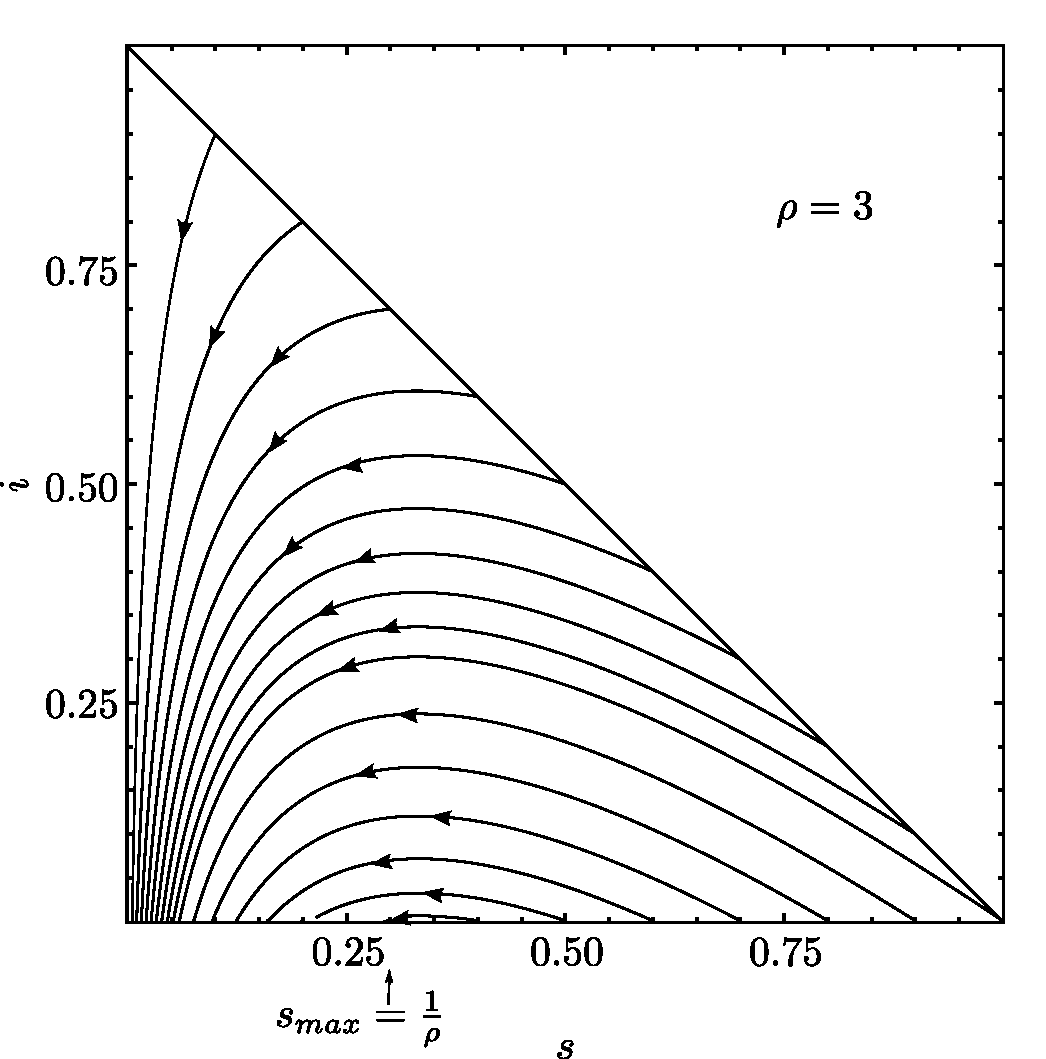
\includegraphics[scale=0.6]{./images/SIR-trial}
\end{center}
\caption{Plano de fases para o modelo SIR. Aqui a vari\'avel $\sigma$ faz o papel de $\rho$.[SUBSTITUIR $\1/\rho$ POR $\rho$]}
\label{fig:SIR-phase-diagram}
\end{figure}

Dado que $r=1-s-i>0$, vemos que as trajet\'orias s\~ao limitadas pelo tri\^angulo mostrado na figura \ref{fig:SIR-phase-diagram}. Podemos calcular tamb\'em o tamanho m\'aximo da epidemia [FALAR ISSO]


Em uma epidemia real pode ser mais f\'acil conhecer o n\'umero de pessoas recuperadas do que de infectadas. Nesse caso, \'e importante conhecer a express\~ao para $dr/dt$. Dividindo a equa\c{c}\~ao \ref{eq:suc-SIR-den} por \ref{eq:rem-SIR-den}, encontramos

\begin{eqnarray}
\frac{ds}{dr}&=&-\frac{r}{\rho}\nonumber \\
&\Rightarrow&s=s_0\exp(r/\rho)
\end{eqnarray}
e a partir de \ref{eq:rem-SIR-den}, temos:
\begin{equation}
\frac{dr}{dt}=\gamma i=\gamma(1-r-s)=\gamma(1-r-s_0 e^{-r/\rho})
\end{equation}  
\'E f\'acil calcular essa express\~ao numericamente se conhecemos todos os par\^ametros, o que, infelizmente n\~ao \'e poss\'ivel em muitos casos. No entanto, podemos fitar os dados se acreditamos que o modelo descreve bem a epidemia, na sequ\^encia temos alguns exemplos.

\begin{figure}[ht!]
\begin{center}
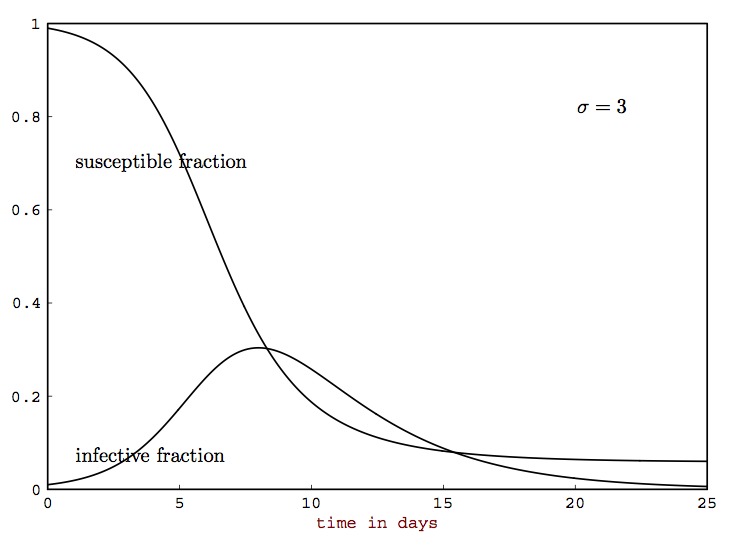
\includegraphics[scale=0.8]{./images/SIR-evolution.pdf}
\end{center}
\caption{Evolu\c{c}\~ao temporal para as vari\'aveis do modelo SIR.}.
\label{fig:SIR-evolution}
\end{figure}


A peste de Bombay foi uma epidemia que aconteceu entre 1905 e 1906. Quase todos os infectados morreram e dai podemos ajustar a taxa de mortalidade com a taxa de remo\c{c}\~ao, podemos tamb\'em usar aproxima\c{c}\~ao mencionada acima. Este caso foi analisado no trabalho original que propos o modelo SIR, por Kermack e McKendrick em 1927. 

\begin{figure}[ht!]
\begin{center}
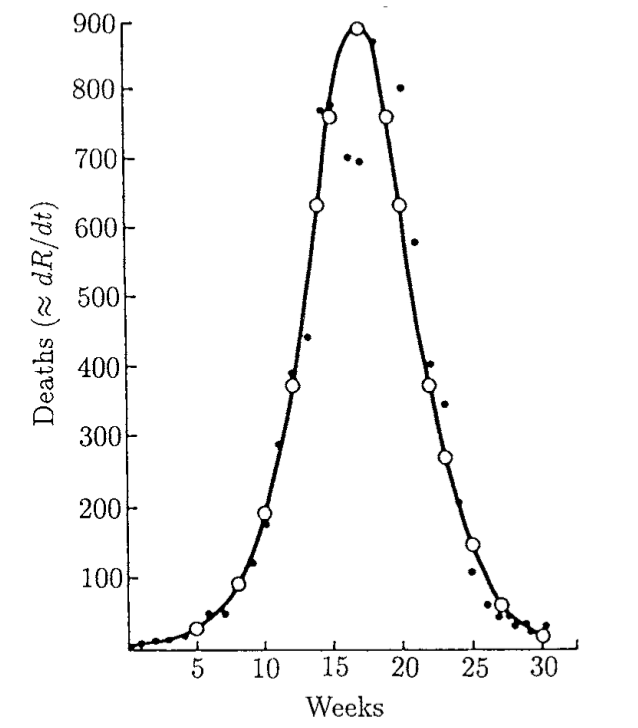
\includegraphics[scale=0.3]{./images/bombay-plague}
\label{fig:Bombay}
\caption{Compara\c{c}\~ao entre os dados (circulos fechados) e o modelo SIR (c\'irculos abertos) para a peste de Bombay.}
\end{center}
\end{figure}

Em uma escola da Inglaterra com 763 alunos aconteceu uma epidemia entre os meses de janeiro e fevereiro de 1978. No total 512 alunos foram infectados durante o surto que parece ter se originado de um \'unico caso. Temos os dados para $i(t)$ e com eles podemos ajustar a curva mostrada na figura \ref{fig:escola}

\begin{figure}[ht!]
\begin{center}
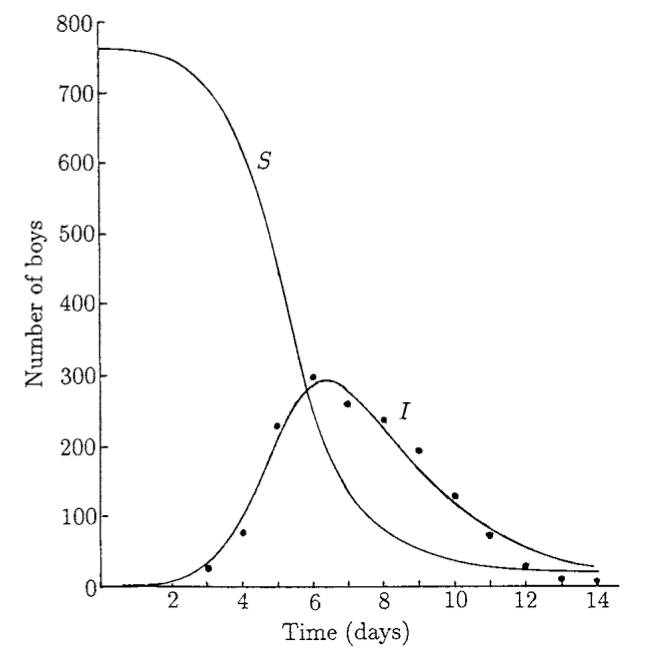
\includegraphics[scale=0.3]{./images/school-plague}
\label{fig:escola}
\caption{Dados para a epidemia de gripe na escola inglesa discutida no texto. Os c\'irculos fechados representam os dados coletados no per\'iodo.}
\end{center}
\end{figure}

Existe na literatura muitos outros modelos de campo m\'edio mais relistas que foram extensivamente estudados. Os modelos que vimos nessa se\c{c}\~ao  s\~ao suficientes para os nossos prop\'ositos. Vamos ver como a inclus\~ao de uma estrutura de rede pode modificar nossos c\'alculos.

\section{Redesin Complexas}
\label{sec:networks}

Os modelos que vimos excluem a discuss\~ao sobre a rede fazendo uso da hip\'otese da aproxima\c{c}\~ao de campo m\'edio. Essa \'e uma aproxima\c{c}\~ao ruim porque no mundo real a probalidade de duas pessoas quaisquer escolhidas ao acaso se encontrarem \'e desprez\'ivel. As pessoas se relacionam apenas com um pequeno n\'umero de conhecidos com regularidade. Esse conjunto de contatos em potencial pode ser representado atrav\'es de uma rede e o tipo de rede pode ter efeitos significantes para a propaga\c{c}\~ao de uma doen\c{c}a. 

A defini\c{c}\~ao mais simples para uma rede \'e um conjunto de pontos conectados por linhas. No jarg\~ao do estudo de redes os pontos s\~ao chamados de v\'ertices ou n\'os. Existem muitos sistemas de interesse f\'isico e tecnol\'ogico que podem ser modelados com redes. Exemplos t\'ipicos s\~ao a internet, cadeias alimentares e redes sociais.

Tradicionalmente esses sistemas s\~ao modelados pelo do grafo aleat\'orio de Erd\H{o}s e R\'enyi (ER). Come\c{c}a-se considerando uma rede com $n$ n\'os. Depois escolhemos cada par de n\'os e os conectamos com uma certa probabilidade $p$. A partir da \'ultima d\'ecada novos modelos passaram a ser considerados, por duas raz\~oes principalmente: o grande aumento de dados relacionados as redes, e o aparecimento de computadores mais potentes e mais baratos. Com isso, se descobriu que as redes reais tem muitas caracter\'isticas que diferem do grafo de ER. Algumas dessas grandezas s\~ao o coeficiente de clustering, o surgimento de correla\c{c}\~oes e a distribui\c{c}\~ao de conectividade.

A distribui\c{c}\~ao de conectividade $P(k)$ \'e definida como a probabilidade de escolher um s\'itio da rede ao acaso e esse s\'itio ter conectividade igual a $k$. Tamb\'em \'e de interesse \'e a distribui\c{c}\~ao condicional $P(k'|k)$, que a probabilidade de que um s\'itio com conectividade $k$ esteja conectado a outro com conectividade $k'$, essa \'ultima distribui\c{c}\~ao caracteriza as correla\c{c}\~oes na rede. 

Em muitos c\'alculos \'e conveniente definir a fun\c{c}\~ao geratriz da distribui\c{c}\~ao

\begin{equation}
g(z)=\sum_{k=0}^{\infty}P(k)z^{k},
\label{eq:geratriz}
\end{equation}
os momentos da distribui\c{c}\~ao de conectividade pode ser obtido de $g(z)$, usando:

\begin{equation}
\langle k^n\rangle=\frac{d^n g}{d(\ln(z))^n}\Bigg|_{z=1}.
\end{equation}

Outra defini\c{c}\~ao importante \'e a de componentes. Um componente \'e definido como um subconjunto de v\'ertices tal que existe pelo menos um caminho de cada membro do conjunto \`a cada um dos outros. 

A distribui\c{c}\~ao de conectividade do grafo de ER \'e, para $n$ grande, uma poissoniana

\begin{equation}
P(k)=\frac{e^{-k}\langle k\rangle}{k!}
\label{eq:dist-ER}
\end{equation}

Essa \'e uma das maiores diferen\c{c}as entre o grafo de ER e as redes sociais reais, que tem como distribui\c{c}\~ao uma lei de pot\^encia:

\begin{eqnarray}
P(k)=\left\{\begin{array}{cl}Ak^{-\gamma}&\quad \mbox{se}\quad k<k_{min}\\0&\quad \mbox{se n\~ao}
\end{array}\right.  
\end{eqnarray}

onde $A$ \'e o fator de normaliza\c{c}\~ao e $k_{min}$ \'e a menor conectividade da distrui\c{c}\~ao. Redes reais tem $2\le \gamma\le 3$, tais redes s\~ao chamadas livres de escala. O modelo de Bar\'abasi se tornou cl\'assico por gerar uma rede livre de escala com expoente igual a 3, generaliza\c{c}\~oes podem ser usadas obter outros expoentes. Na pr\'oxima se\c{c}\~ao descrevemos um algoritmo simples para se gerar uma rede com a distribui\c{c}\~ao de conectividade que desejarmos.


\subsection{Modelo Configuracional}

O modelo configuracional \'e um dos modelos de grafo alet\'orio generalizado mais famosos. Nesse modelo, n\~ao especificamos a distribui\c{c}\~ao $P(k)$, e sim a sequ\^encia de conectividade que \'e o conjunto de $\{k_1, k_2, ...\}$ de conectividade de cada v\'ertice. Note que assim tamb\'em fixamos o n\'umero de liga\c{c}\~oes do grafo $m=\frac{1}{2}\sum k_i$. A rede \'e constru\'ida da seguinte maneira: suponha que especificamos a conectividade de cada um dos v\'ertices, atribu\'indo \'a cada um deles um n\'umero $k_i$ de liga\c{c}\~oes abertas. Depois escolhemos duas liga\c{c}\~oes abertas e as ligamos da maneira ilustrada na figura (\ref{fig:config-model}). Esse processo \'e repetido at\'e que cada um dos v\'ertices tenha a conectividade atribu\'ida na primeira etapa. 

\begin{figure}[ht!]
\begin{center}
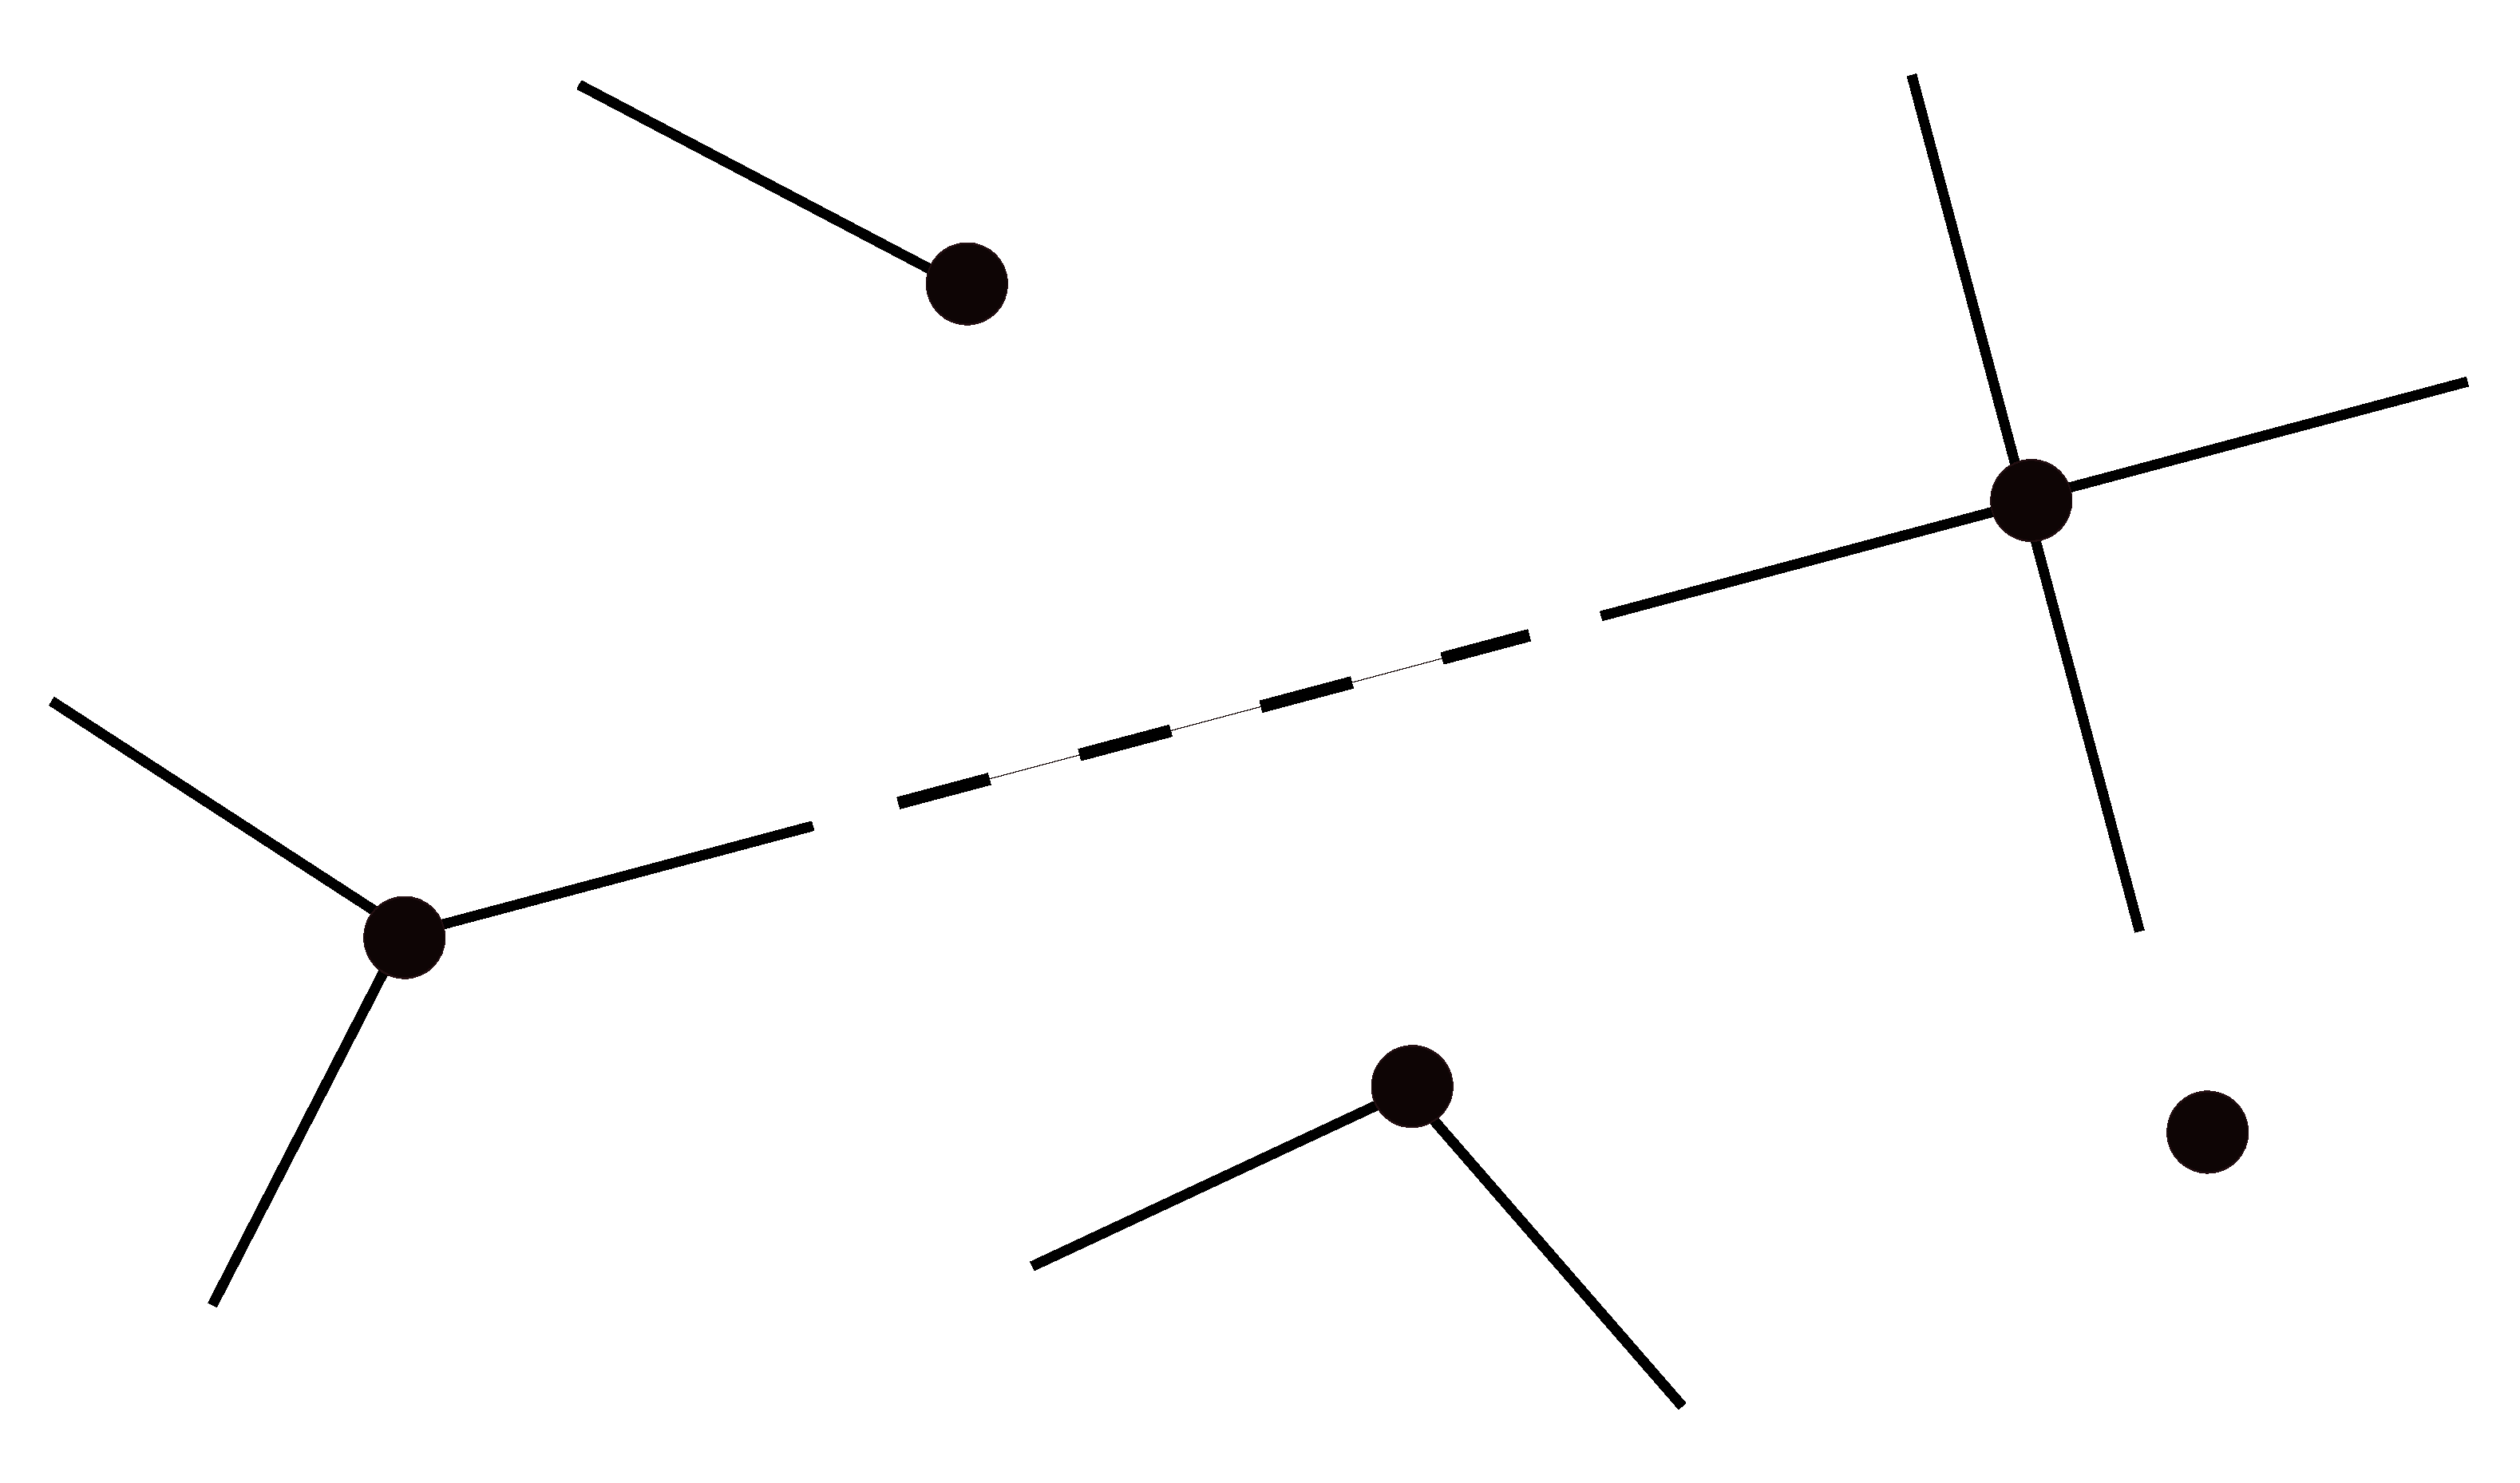
\includegraphics[scale=0.15]{./images/config-model.pdf}
\end{center}
\caption{Atribu\'imos \'a cada um dos v\'ertices um certo n\'umero de liga\c{c}\~oes abertas. Depois cada par de liga\c{c}\~oes abertas \'e conectado formando liga\c{c}\~oes (linha pontilhada).}
\label{fig:config-model}
\end{figure}

Esse modelo fornece uma forma de gerar redes no computador com uma dada distribui\c{c}\~ao e permite fazer alguns c\'alculos anal\'icos. Por exemplo, suponha que escolhemos um dos v\'ertices ao acaso e seguimos uma de suas liga\c{c}\~oes at\'e o v\'ertice na outra ponta. Qual a probabilidade de que esse v\'ertice tenha conectividade $k$? No modelo configuracional a probabilidade de uma liga\c{c}\~ao do v\'ertice que escolhemos terminar em qualquer uma das outras pontas \'e a mesma. Excluindo a ponta de origem existem  $2m-1$ outras pontas na rede e $k$ delas est\~ao conectadas a qualquer v\'ertice com conectividade $k$, da\'i a liga\c{c}\~ao que escolhemos tem probabilidade $k/2m$, no limite de $m$ grande, de terminar em um determinado v\'ertice com conectividade $k$. Dado que existem no total $nP(k)$ v\'ertices com conectividade $k$ a probabilidade de uma liga\c{c}\~ao estar em um qualquer um dos v\'ertices com conectividade $k$ \'e:

\begin{equation}
\frac{k}{2m}\times P(k)=\frac{kP(k)}{\langle k\rangle}
\end{equation}
onde $\langle k\rangle$ \'e a conectividade m\'edia da rede e usamos que  $2m=n\langle k\rangle$. 

A probabilidade de alcan\c{c}ar um v\'ertice com $k+1$ liga\c{c}\~oes \'e chamada de distribui\c{c}\~ao de conectividade em excesso e \'e definida por

\begin{equation}
q_k=\frac{(k+1)P(k+1)}{\langle k\rangle}
\label{eq:excess-degree}
\end{equation}

\section{Modelo SIR - Comportamento assint\'otico}
\label{subsec:SIR-perc}

Vamos considerar agora que todo o processo de transmiss\~ao da doen\c{c}a acontece usando a rede de contatos. Definimos a taxa de transmiss\~ao ou infec\c{c}\~ao como sendo a probabilidade por unidade de tempo que a doen\c{c}a seja transmitada de um indiv\'iduo infectado para um suscept\'ivel que estejam conectados por uma liga\c{c}\~ao da rede. Essa taxa \'e denotada por $\beta$ como nos modelos de campo m\'edio. Note, que as defini\c{c}\~oes n\~ao s\~ao exatamente as mesmas dado que nos modelos de campo m\'edio corresponde a taxa com que indiv\'iduos infectados se encontram com qualquer outro membro da popula\c{c}\~ao e aqui diz respeito a taxa de contato entre dois indiv\'iduos. 

A taxa de infec\c{c}\~ao \'e uma propriedade da doen\c{c}a, certas doen\c{c}as s\~ao mais infecciosas que outras, mas tamb\'em depende do 
comportamento da popula\c{c}~ao que se est\'a estudando. 

Para um dado valor de $\beta$, podemos definir modelos para epidemias na rede. Os modelos SI e SIR que vimos anteriormente tem suas vers\~oes na rede. Vamos come\c{c}ar com o modelo SI que \'e mais simples. Cada s\'itio de uma rede com $n$ n\'os corresponde a um membro da popula\c{c}\~ao. Inicialmente, em $t=0$, uma frac\c{c}\~ao $i_0$ desses v\'ertices est\~ao infectados, inclusive podemos usar a condi\c{c}\~ao inicial de que s\'o um v\'ertice est\'a infectado, esse v\'ertice \'e chamado de semente. Com uma probabilidade por unidade de tempo $\beta$ esses indiv\'iduos espalham a doen\c{c}a para seus vizinhos e a doen\c{c}a se espalha pela rede. 

\begin{figure}[ht!]
\begin{center}
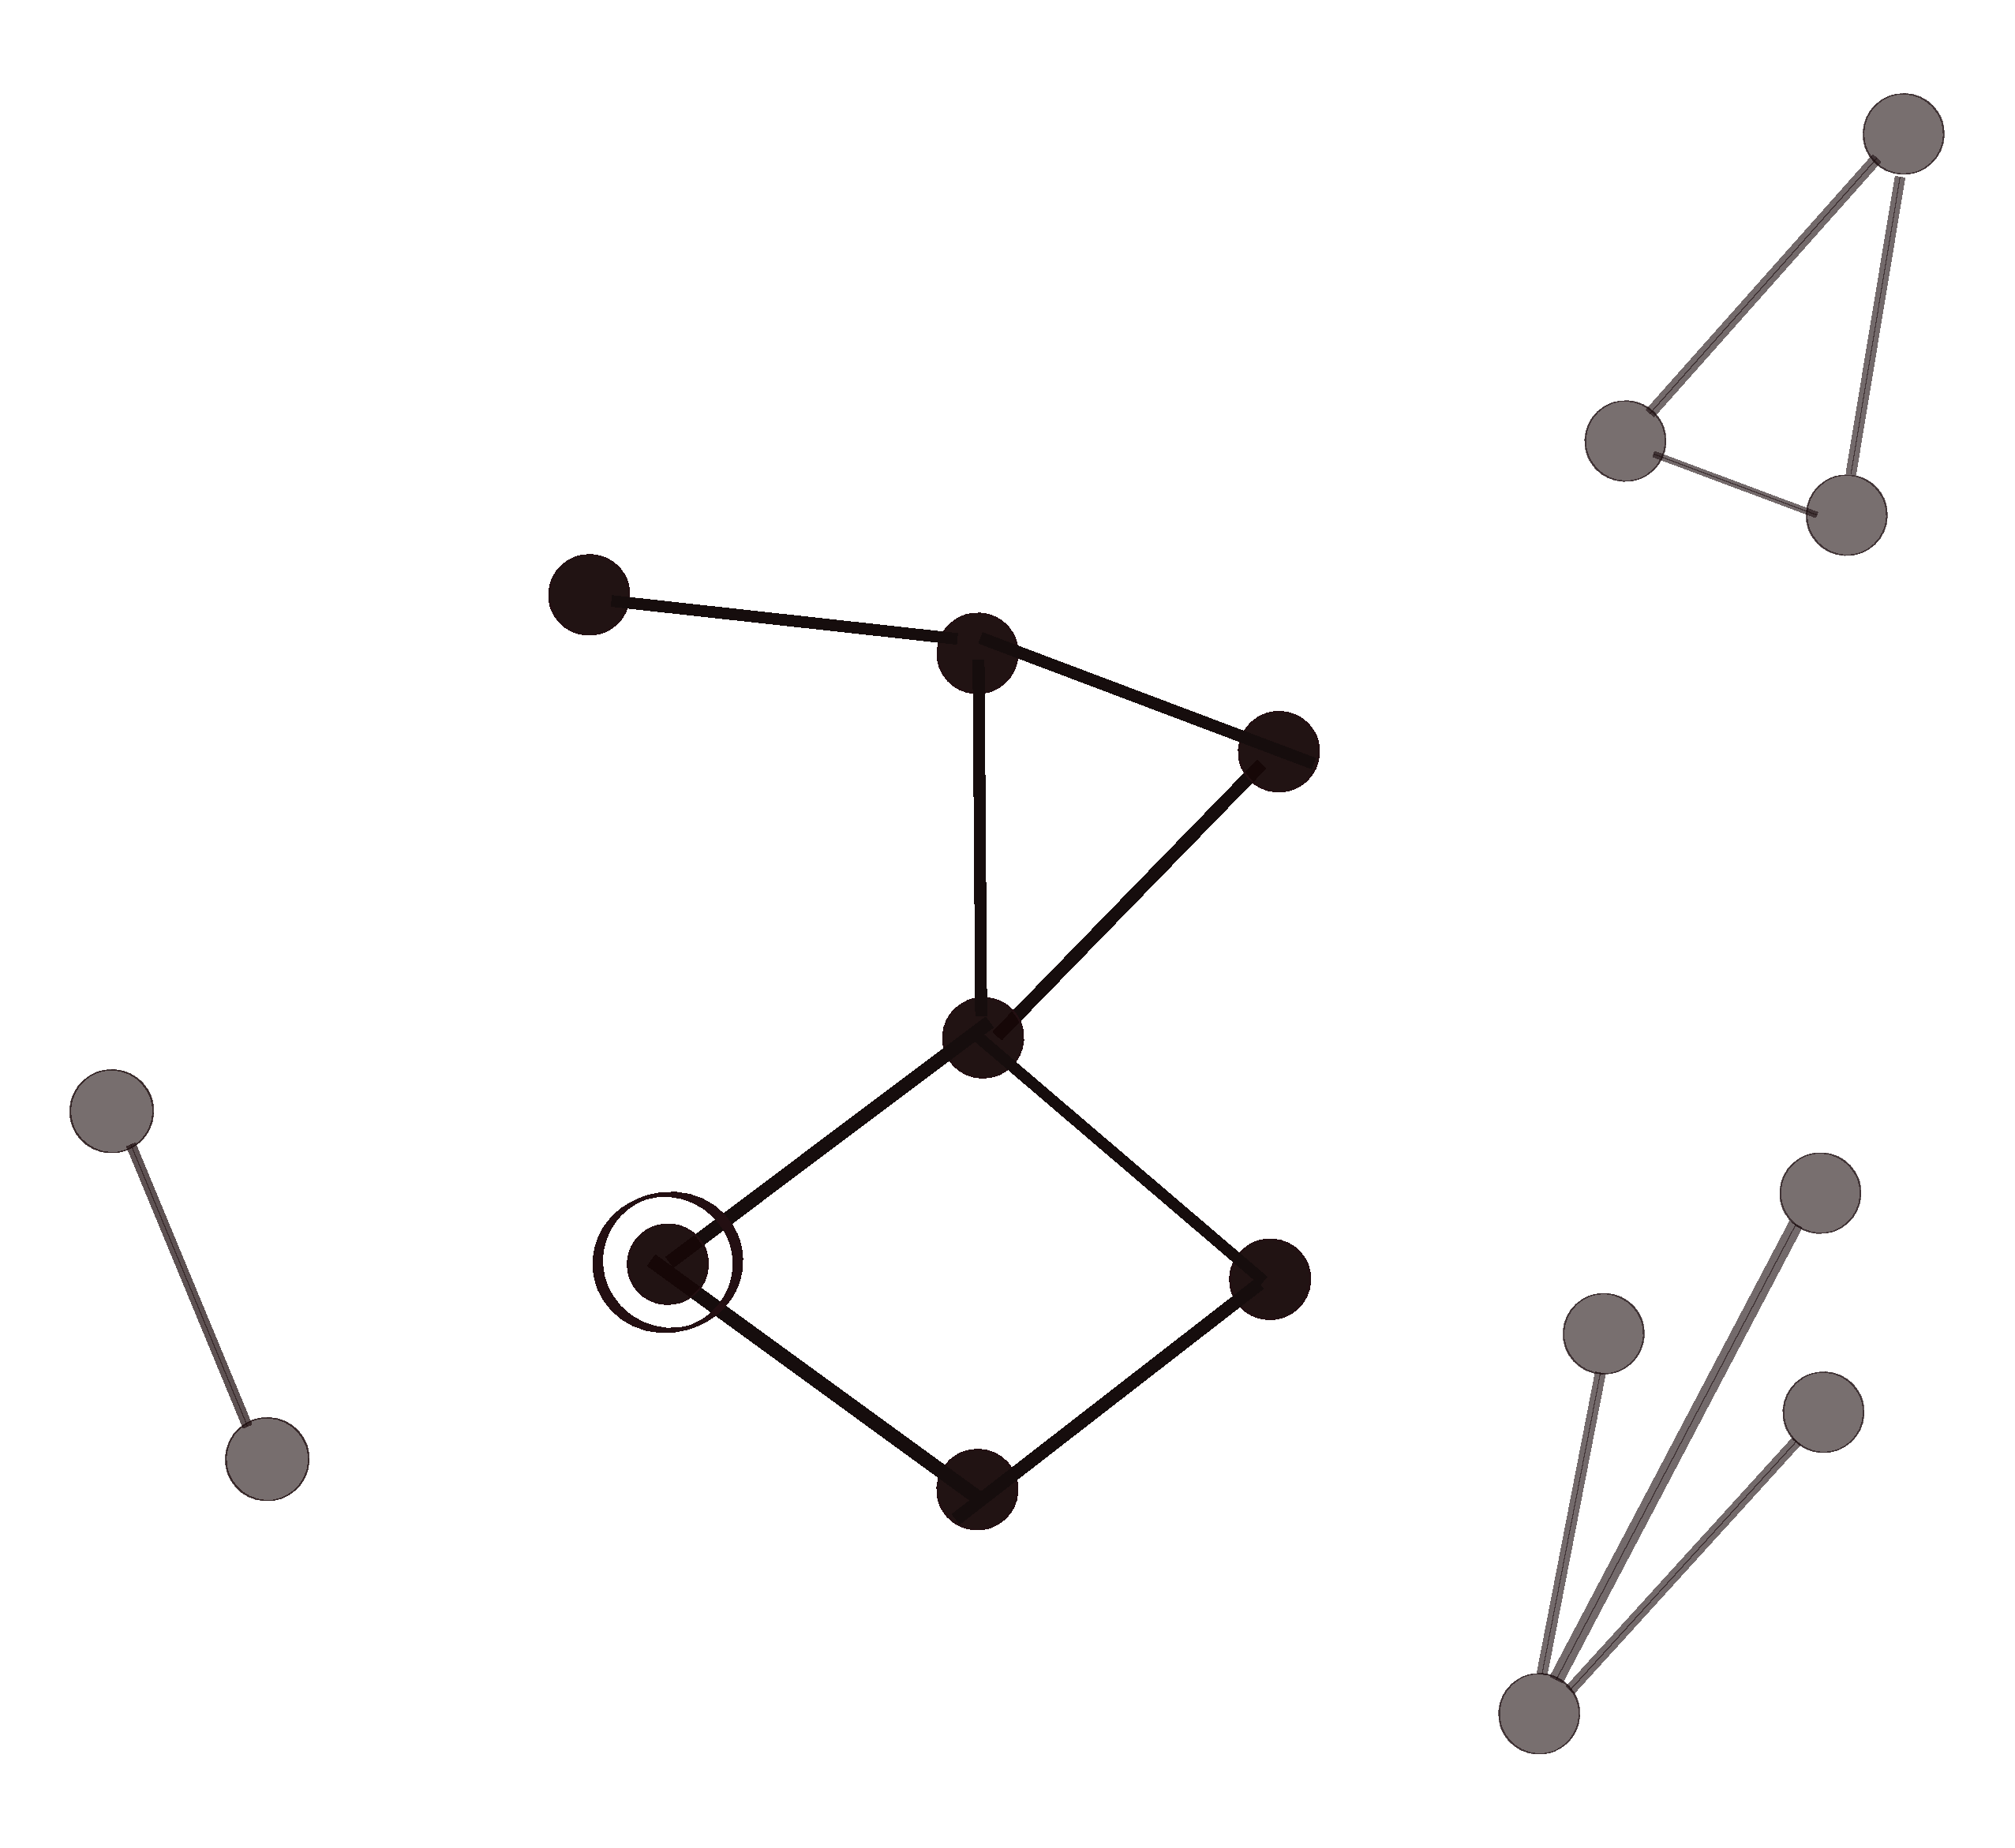
\includegraphics[scale=0.2]{./images/SI-model}
\label{fig:SI-model}
\caption{Modelo SI na rede.}
\end{center}
\end{figure}

\'E muito complicado resolver esse modelo de maneira geral, mas com rela\c{c}\~ao \`as propriedades assint\'oticas o modelo \'e trivial. Dado que uma vez no estado infectado a pessoa permanece infectada para sempre. No limite em que $t\to \infty$ todos os indiv\'iduos que podem ser infectados ser\~ao infectados, independente dos valores de $\beta$ e $i_0$. S\'o temos uma condi\c{c}\~ao: cada v\'ertice tem que estar conectado com pelo menos um v\'ertice infectado por pelo menos um caminho.  

Dito isso, todos os v\'ertices que pertencem ao mesmo componente que o v\'ertice que deu origem a epidemia ser\~ao eventualmente infectados. A maioria das redes sociais reais e tamb\'em aquelas feitas no computador, tem uma componente que cont\'em a grande maioria dos v\'ertices e alguns componentes menores. Se escolhemos a semente ao acaso dentre todos os v\'ertices da rede, a probalidade dessa semente pertencer a maior componente \'e igual a $S$, a fra\c{c}\~ao de rede ocupada pela componente maior, e nesse caso temos um grande n\'umero de indiv\'iduos infectados, caso contr\'ario a epidemia fica restrita a uma fra\c{c}\~ao pequena da popula\c{c}\~ao. N\~ao podemos predizer com exatid\~ao o tamanho da epidemia, a menos que saibamos em qual componente caiu a semente. Esse comportamento \'e diferente dos modelos de campo m\'edio, que prediz os mesmos resultados dado um conjunto de par\^ametros. Temos a introdu\c{c}\~ao de um elemento estoc\'astico. O comportamento do sistema depende da escolha da semente e da estrutura da rede e podemos ter uma sa\'ida diferente mesmo usando a mesma rede e os mesmos par\^ametros. 

A situa\c{c}\~ao \'e bem mais interessante quando consideramos o modelo SIR numa rede. No modelo SIR, os indiv\'iduos permanecem infectados somente durante um intervalo finito de tempo ap\'os o qual eles se recuperam. N\~ao \'e verdade que um v\'ertice suscept\'ivel com um vizinho infectado acabe sendo infectado. Pode ser que ele nunca venha a pegar a doen\c{c}a. A probabilidade de que haja infe\c{c}\~ao ap\'os qualquer intervalo de tempo $dt$ \'e $\beta dt$ e de que n\~ao haja \'e $(1-\beta dt)$. Portanto, a probabilidade de que uma infe\c{c}\~ao n\~ao ocorra em um intervalo de tempo $\tau$ finito \'e igual a 

\begin{equation}
\lim_{dt\to 0}(1-\beta dt)^{\tau/dt}=e^{-\beta\tau}
\end{equation}

Por fim, a probabilidade de que a doen\c{c}a seja transmitida \'e

\begin{equation}
\phi=1-e^{-\beta\tau}
\end{equation}

Por simplicidade vamos supor que $\phi$ \'e o mesmo para toda popula\c{c}\~ao. Vamos supor que cada indi\'viduo infectado permanece infectado durante a mesma quantidade de tempo. Cada indiv\'iduo suscept\'ivel tem a mesma probabilidade de pegar a doen\c{c}a de um de seus vizinhos infectados. 

Para estudar as propriedades assint\'oticas do modelo, vamos usar fazer a formula\c{c}\~ao proposta em \cite{Grassberger:1983tj}, onde cada uma das liga\c{c}\~oes \'e considerada ``colorida"$\;$ (ou ocupada) com probalidade $\phi$ ou vazia com probabilidade $1-\phi$. Esse problema \'e an\'alogo ao problema de percola\c{c}\~ao por liga\c{c}\~oes, onde uma fra\c{c}\~ao $\phi$ das liga\c{c}\~oes escolhida ao acaso est\'a ocupada. O grupo de v\'ertices conectados por liga\c{c}\~oes coloridas \'e chamado de \textit{cluster}.

As liga\c{c}\~oes fechadas representam contatos pelos quais a doen\c{c}a pode ser transmitida se alcan\c{c}ar uma das pontas dessa liga\c{c}\~ao, se a doen\c{c}a n\~ao alcan\c{c}ar uma dessas pontas n\~ao ocorrer\'a transmiss\~ao da doen\c{c}a. 

Para valores pequenos de $\phi$ existem poucas liga\c{c}\~oes coloridas as quais se agrupam em pequenos clusters disconexos. \`A medida que $\phi$ aumenta esses cluster menores se agrupam formando um cluster que tem o tamanho da ordem de $n$, chamado de cluster gigante ou cluster percolante. Se $\phi$ aumenta ainda mais o cluster gigante continua aumentando e atinge seu valor m\'aximo quando $\phi=1$. Contudo, n\~ao necessariamente esse cluster vai englobar todos os elementos da rede porque \'e limitado pelo tamanho da maior componente, que por sua vez pode ser menor que $n$. A transi\c{c}\~ao em que aparece o cluster gigante \'e chamada de transi\c{c}\~ao de percola\c{c}\~ao. 

Voltando para o espalhamento de doen\c{c}as: para $\phi$ pequeno, a semente pertence a um dos clusters pequenos e n\~ao h\'a epidemia. Suponha agora que $\phi>\phi_c$ e existe um cluster percolante, nesse caso existe a possibilidade de uma epidemia. O cluster gigante ocupa uma fra\c{c}\~ao $S$ da rede e portanto existe uma probabilidade $S$ que a semente caia nesse cluster dando origem a uma epidemia. A medida em que $\phi$ aumenta, aumenta tamb\'em a probabilidade de haver uma epidemia. Portanto a transi\c{c}\~ao de percola\c{c}\~ao por liga\c{c}\~oes correspondente ao limiar epid\^emico para uma doen\c{c}a ocorrendo na mesma rede.

\begin{figure}[ht!]
\begin{center}
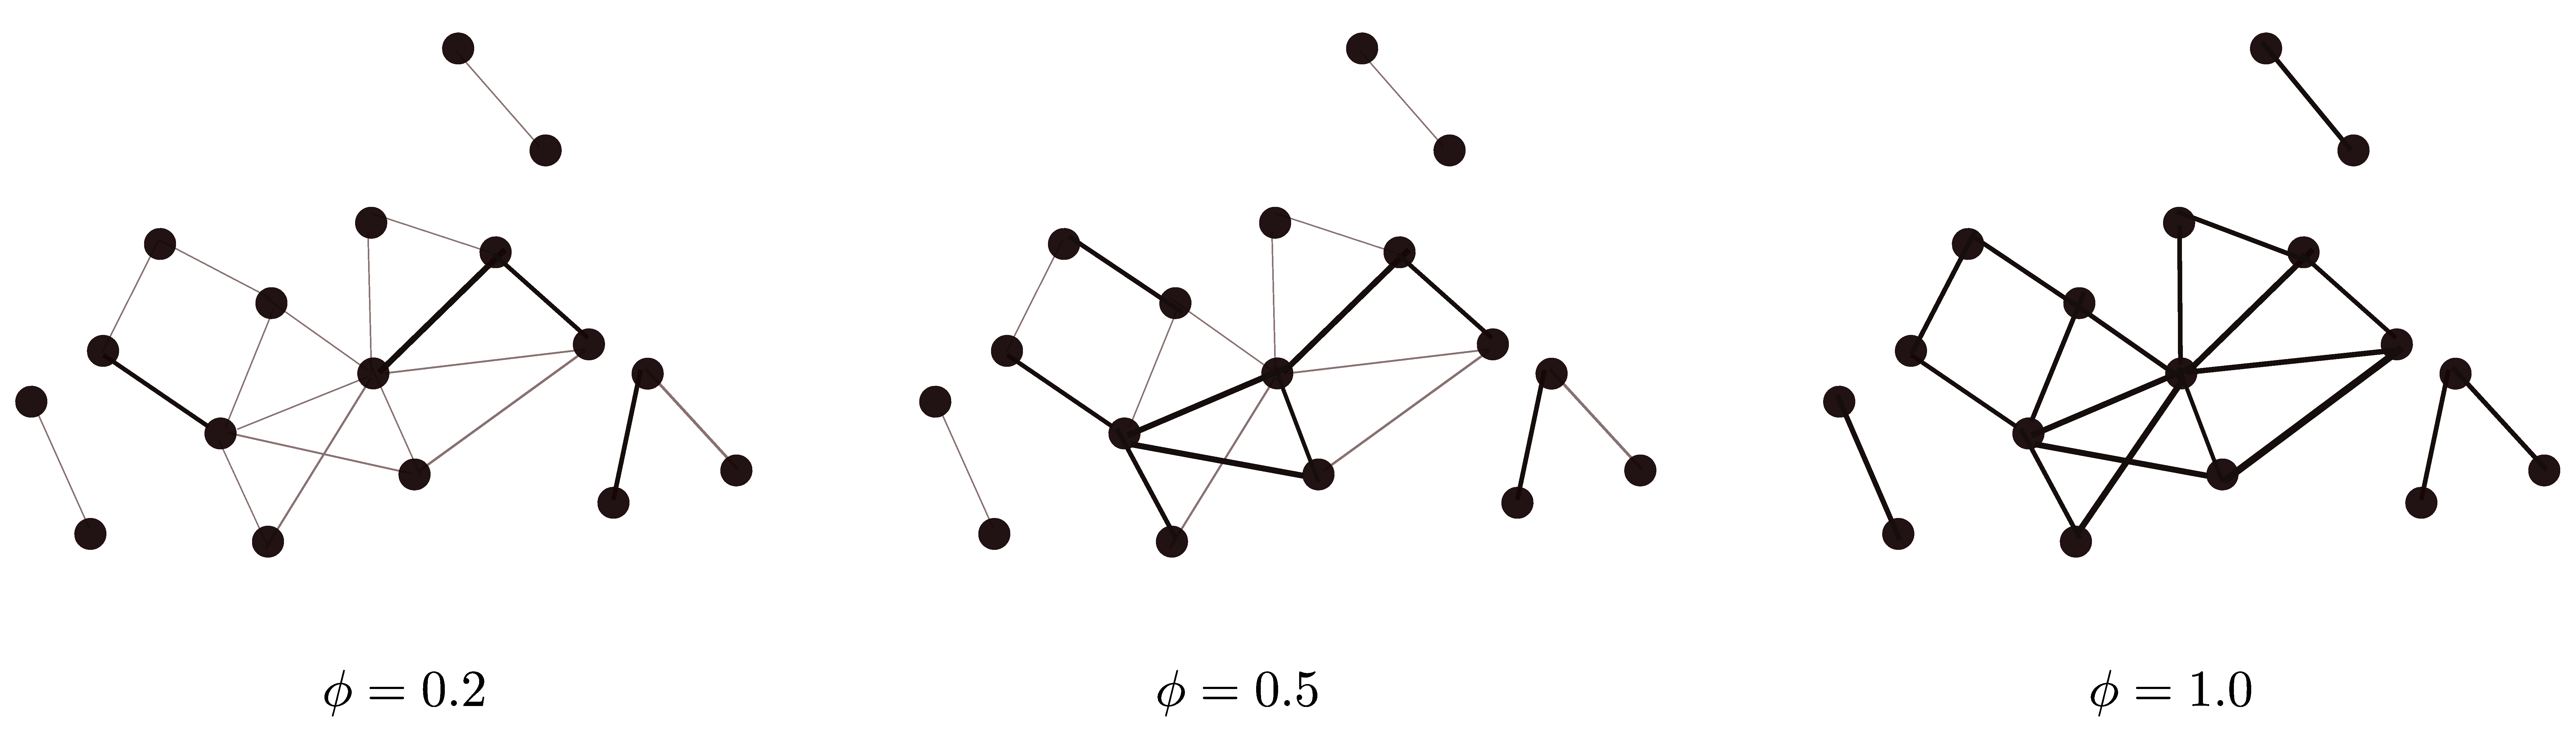
\includegraphics[scale=0.1]{./images/perc.pdf}
\label{fig:perc}
\caption{Percola\c{c}\~ao por liga\c{c}\~oes.}
\end{center}
\end{figure}

Considere ent\~ao o modelo SIR em uma rede montada com o modelo configuracional com distribui\c{c}\~ao $P(k)$. Considere que $u$ \'e a probabilidade m\'edia de que um dado v\'ertice n\~ao esteja conectado ao cluster percolante por uma de suas liga\c{c}\~oes. Existem duas possibilidades: ou essa liga\c{c}\~ao est\'a vazia, o que acontece com probabilidade $1-\phi$, ou est\'a ocupada mas n\~ao pertence ao cluster percolante. A \'ultima op\c{c}\~ao ser\'a verdade se o v\'ertice n\~ao est\'a conectado ao cluster percolante por nenhuma de suas liga\c{c}\~oes, o que tem probalidade $u^k$, no caso em que o v\'ertice tem $k$ liga\c{c}\~oes. Somando as duas possibilidades temos que a probabilidade total ser\'a $(1-\phi+\phi u^{k})$, onde valor de $k$ tem distribui\c{c}\~ao \ref{eq:excess-degree}. Fazendo a m\'edia sobre todos os valores de $k$, ficamos com:

\begin{equation}
u=1-\phi+\phi\sum_{k=0}^{\infty}q_ku^{k}=1-\phi+\phi g_1(u)
\label{eq:not-connect}
\end{equation}
na equa\c{c}\~ao acima $g_1(u)$ \'e a fun\c{c}\~ao geratriz de $q_k$.

A probabilidade de que um  v\'ertice com $k$ liga\c{c}\~oes n\~ao fa\c{c}a parte do cluster percolante ser\'a $u^k$, a m\'edia dessa grandeza sobre todos os elementos da rede \'e igual \`a $1-S$ e portanto:

\begin{equation}
S=1-\sum_{k=0}^{\infty}P(k)u^k=1-g_0(u)
\label{eq:giant-cluster}
\end{equation}

As equa\c{c}\~oes \ref{eq:not-connect} e \ref{eq:giant-cluster} fornecem a solu\c{c}\~ao para o nosso problema. No entanto, n\~ao conhecemos a forma exata para $g_1(k)$, mas podemos encontrar a solu\c{c}\~ao ainda assim usando um m\'etodo gr\'afico. 

\begin{figure}[ht!]
\begin{center}
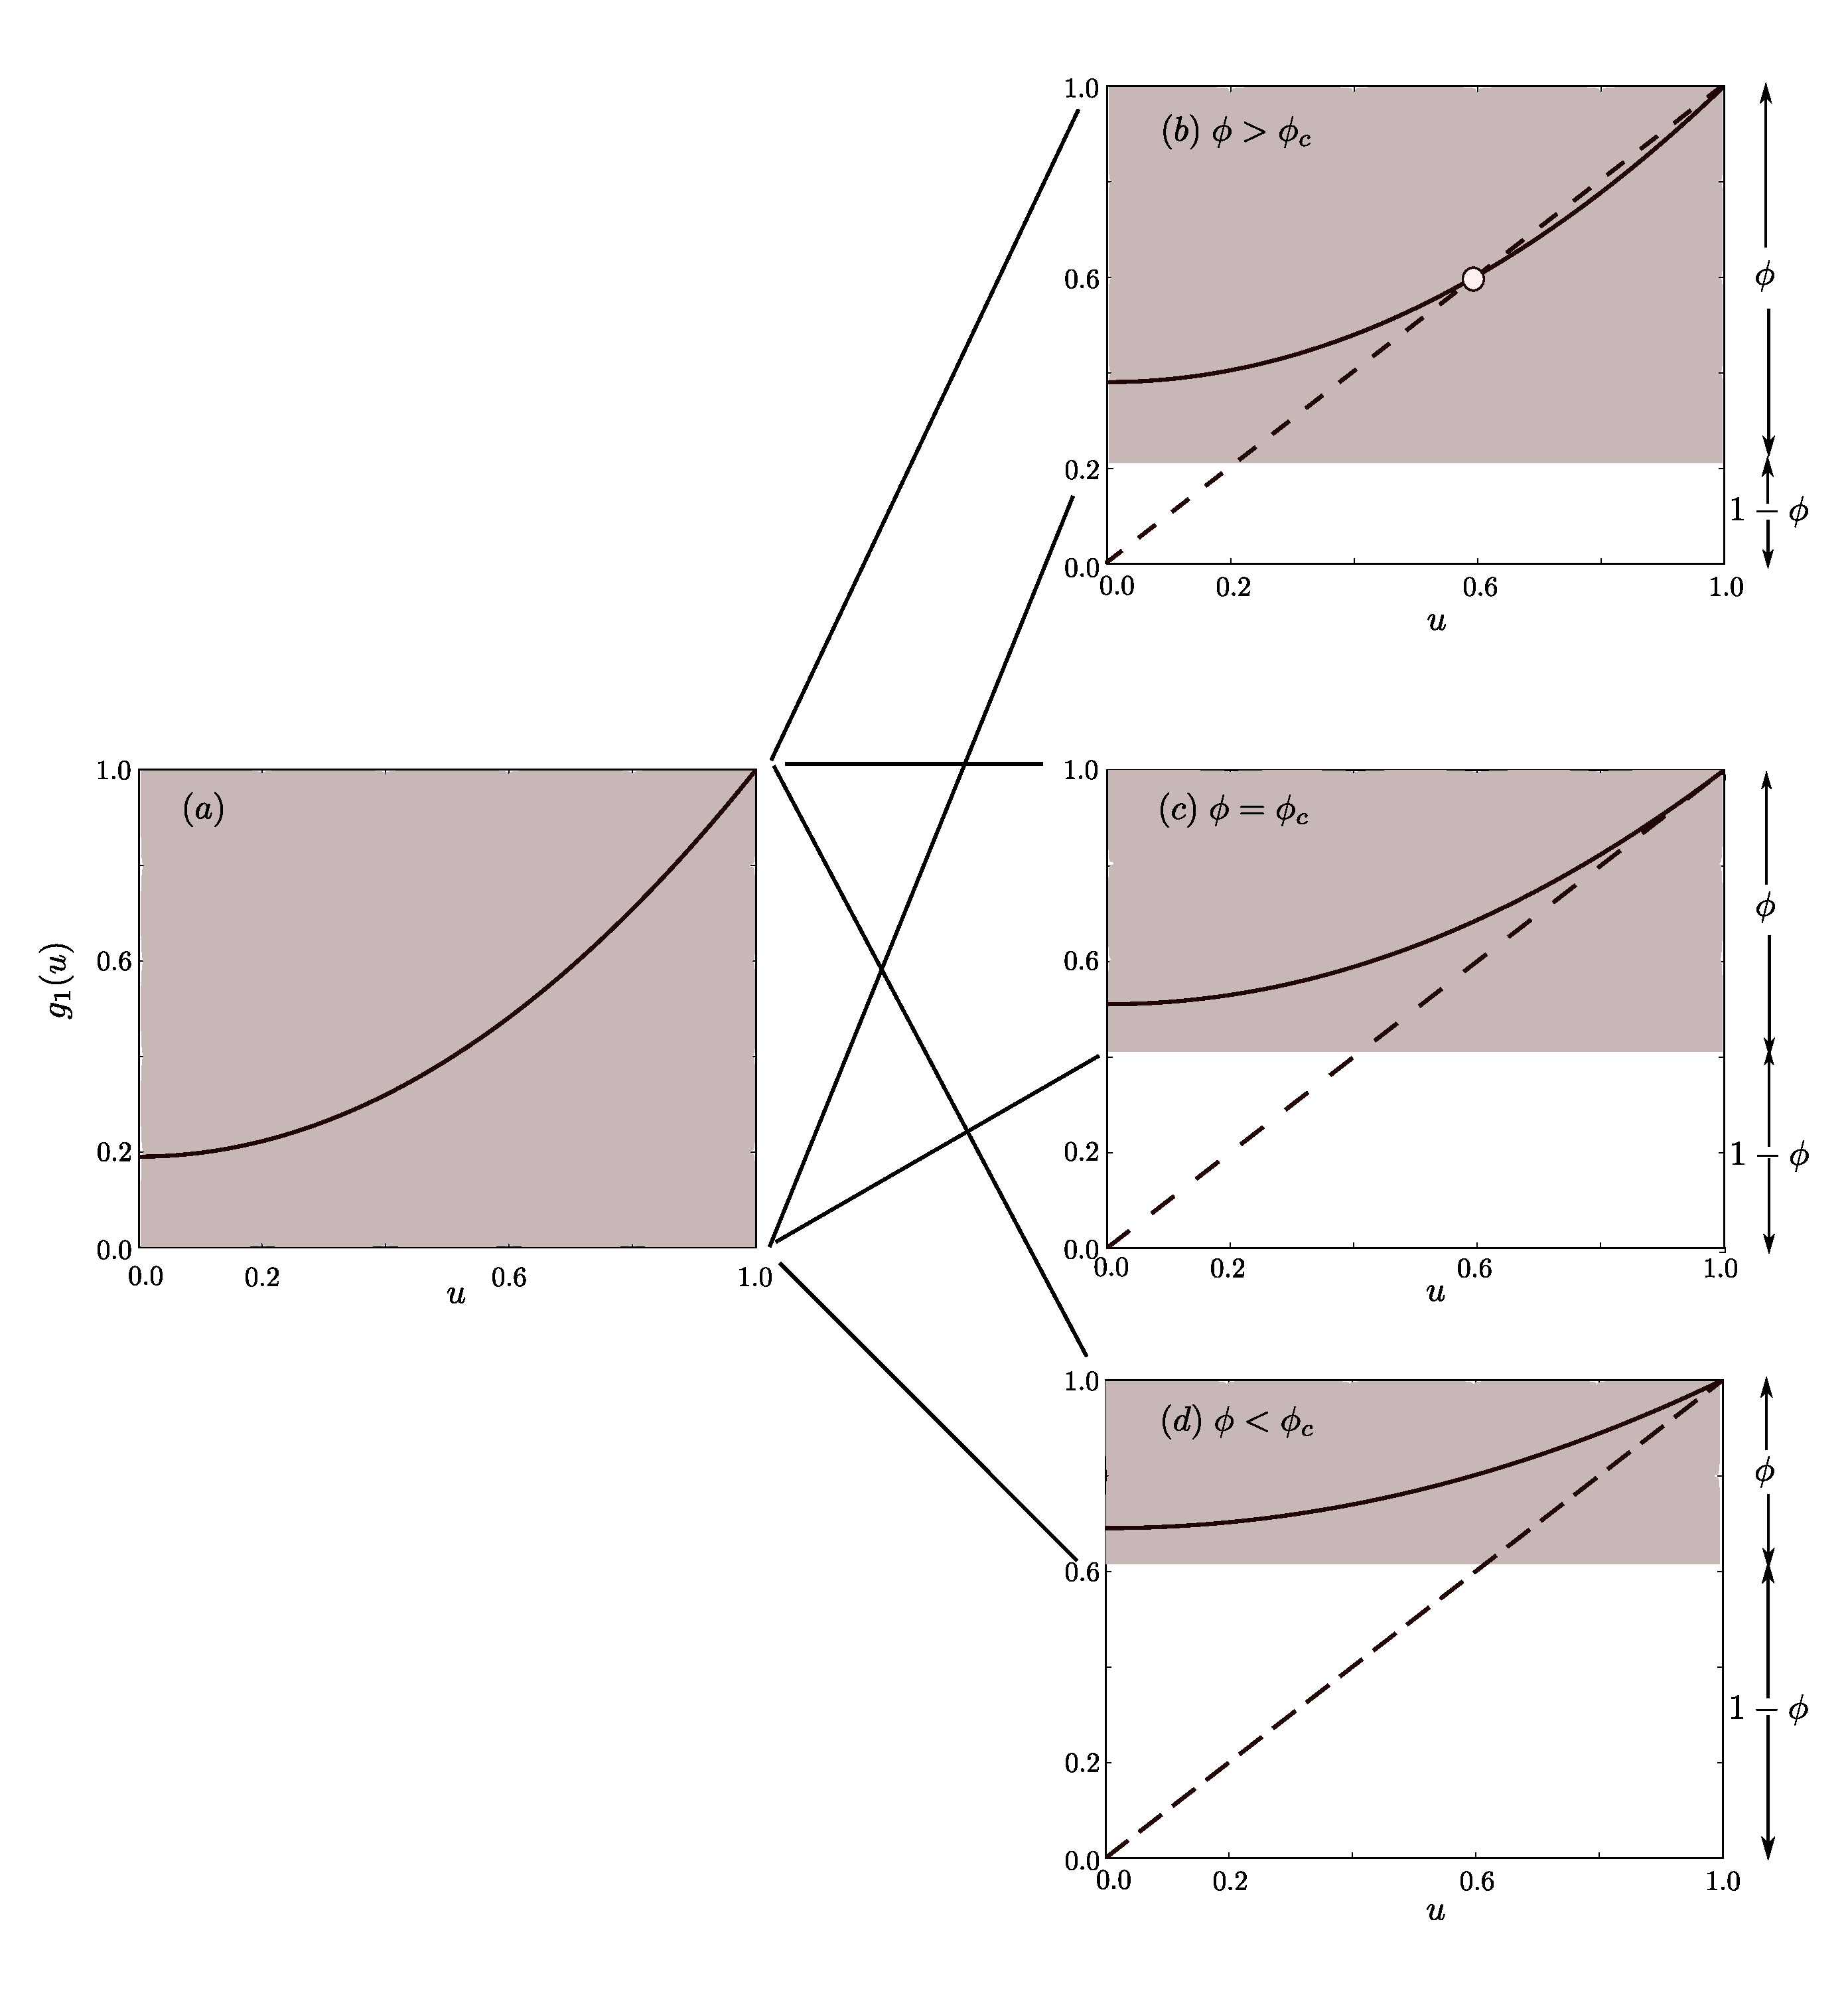
\includegraphics[scale=0.35]{./images/plot-geratriz.pdf}
\label{fig:plot-geratriz}
\caption{M\'etodo gr\'afico usado para resolver a equa\c{c}\~ao \ref{eq:not-connect}.}
\end{center}
\end{figure}

A fun\c{c}\~ao caracter\'istica $g_1(x)$ \'e um polin\^omio com todos os coeficientes n\~ao negativos, e da\'i \'e uma fun\c{c}\~ao crescente com todas as derivadas positivas como ilustrado na figura (\ref{fig:plot-geratriz}). A fun\c{c}\~ao \ref{eq:not-connect} pode ser obtida comprimindo $g_1$ por um fator $\phi$ e depois somando $1-\phi$. As interse\c{c}\~oes com a curva $y=u$ nos fornece as solu\c{c}\~oes. 

Para um valor grande de $\phi$ existem duas solu\c{c}\~oes, uma delas, $u=1$, \'e trivial e sempre acontece. A outra solu\c{c}\~ao nos d\'a o tamanho do maior cluster. 

Se $u$ \'e muito pequeno s\'o existe a solu\c{c}\~ao trivial. O ponto de transi\c{c}\~ao acontece quando a curva $y=1-\phi+\phi g_1(u)$ \'e tangente a reta $y=u$, ou seja, quando


\begin{equation}
\left[\frac{d}{du}(1-\phi+\phi g_1(u))\right]_{u=1}=1
\end{equation}
calculando essa derivada, obter o valor do ponto $\phi_c$ onde ocorre a transi\c{c}\~ao,
\begin{equation}
\phi_c=\frac{1}{g'_1(1)}.
\label{eq:phi-c1}
\end{equation}

Usando as equa\c{c}\~oes \ref{eq:geratriz} e \ref{eq:excess-degree}:

\begin{eqnarray}
g'_1(1)&=&\frac{1}{\langle k\rangle}\sum_{k=0}^{\infty}k(k+1)p_{k+1}=\frac{1}{\langle k\rangle}\sum_{k=0}^{\infty}k(k-1)p_{k}\nonumber \\
\phantom{g'_1(1)}&=&\frac{\langle k^2\rangle-\langle k\rangle}{\langle k\rangle}
\end{eqnarray}
substituindo em \ref{eq:phi-c1}, ficamos com

\begin{equation}
\phi_c=\frac{\langle k\rangle}{\langle k^2\rangle-\langle k\rangle}
\label{eq:phi-c2}
\end{equation}
ou, em termos das vari\'aveis originais, $\beta$ e $\tau$:

\begin{equation}
\beta \tau=-\ln(1-\phi_c)=\ln\left(\frac{\langle k^2\rangle-\langle k\rangle}{\langle k^2\rangle-2\langle k\rangle}\right)
\label{eq:beta-tau}
\end{equation}
para valores de $\phi$ abaixo de $\phi_c$ a preval\^encia de epidemia \'e nula, e acima de $\phi_c$ a doen\c{c}a atinge uma frac\c{c}\~ao finita da popula\c{c}\~ao. Um caso importante a ser considerado s\~ao as distribui\c{c}\~oes com lei de pot\^encia. Se temos uma rede livre de escala, ou seja, com expoente entre 2 e 3, ent\~ao $\phi_c=0$, porque o segundo momento diverge quando $N\to\infty$ mas a m\'edia permanece finita. Portanto nesse caso sempre temos uma epidemia, mesmo se a taxa de transiss\~ao da doen\c{c}a for muito pequena. Por outro lado para redes reais que tem $N$ finito, existe um limiar que embora pequeno \'e diferente de zero.


\section{Aproxima\c{c}\~ao por conectividade}

A aproxima\c{c}\~ao introduzida na refer\^encia \cite{MORENO:2002bb} assume que cada v\'ertice com a mesma conectividade tem a mesma probabilidade de estar infectado em um dado instante de tempo. Vamos definir $s_k(t)$, $i_k(t)$ e $r_k(t)$ como sendo a probabilidade de que um s\'itio com conectividade $k$, esteja no estado suscept\'ivel, infectado ou removido, respectivamente, no tempo $t$.

Considere um v\'ertice qualquer da rede, para se tornar infectado esse v\'ertice tem que ter pego a doen\c{c}a de um dos seus vizinhos, ou seja, esse s\'itio deve ter uma liga\c{c}\~ao que aponte para um v\'ertice infectado. Vimos na se\c{c}\~ao \ref{sec:networks} que a probabilidade de que uma dada liga\c{c}\~ao aponte para um s\'itio com conectividade $k$ \'e proporcional \'a $kP(k)$. Portanto a probabilidade de que uma dada liga\c{c}\~ao aponte para um s\'itio infectado ser\'a:

\begin{equation}
\Theta(t)=\frac{\sum_k k P(k)i_k(t)}{\sum_k k P(k)}=\frac{\sum_k kP(k)i_k(t)}{\langle k\rangle}	
\end{equation}

Se o vizinho de um dado v\'ertice est\'a infectado, ent\~ao a probabilidade de que a doen\c{c}a seja transmitida para esse v\'ertice em um intervalo de tempo $dt$ \'e $\beta dt$. A probabilidade de um n\'o pegar a doen\c{c}a de um dos vizinhos ser\'a $\beta \Theta(t)dt$ e por fim a probabilidade total de transmiss\~ao da doen\c{c}a por qualquer um dos vizinhos \'e $\beta k\Theta(t)dt$. Em adi\c{c}\~ao exigimos que o pr\'oprio s\'itio em considera\c{c}\~ao seja suscept\'ivel o que tem probabilidade $s_k$ de acontecer. Portanto a taxa de mudan\c{c}a em $s_k$ \'e dada por

\begin{equation}
\frac{ds_k}{dt}=-\beta ks_k\Theta(t)
\label{eq:suc-degree}
\end{equation}
as outras probabilidades evoluem segundo as equa\c{c}\~oes:

\begin{equation}
\frac{di_k}{dt}=-\beta ks_k\Theta(t)-\gamma i_k
\end{equation}
e 
\begin{equation}
\frac{dr_k}{dt}=\gamma i_k
\end{equation}
as condi\c{c}\~oes iniciais s\~ao $r_k(0)=0$, $i_k(0)=i_k^0$ e $s_k(0)=1-i_k^0$.  Podemos fazer tamb\'em $s(0)=1$ assumindo que o tamanho do sistema \'e grande e a frac\c{c}\~ao de infectados \'e pequena. Definimos a probabilidade de que um vizinho esteja no estado $r$ como

\begin{equation}
\theta=\frac{\sum_k kP(k)r_k(t)}{\langle k\rangle}.
\end{equation}
Derivando essa express\~ao em rela\c{c}\~ao ao tempo, encontramos:
\begin{equation}
\frac{d\theta}{dt}=\frac{1}{\langle k\rangle}\sum_k kP(k)\frac{dr_k}{dt}=\gamma \Theta,
\label{eq:theta-der1}
\end{equation}
substituindo essa express\~ao em \ref{eq:suc-degree} e integrando:

\begin{equation}
s_k=e^{-\beta k \theta/\gamma}
\end{equation}
e voltando para a express\~ao \ref{eq:theta-der1}
\begin{eqnarray}
\frac{d\theta}{dt}&=&\frac{\gamma}{\langle k\rangle}\sum_k kP(k)i_k\nonumber \\
&=&\frac{\gamma}{\langle k\rangle}\sum_k kP(k)(1-r_k-s_k)\nonumber\\
&=&\gamma-\gamma\theta-\frac{\gamma}{\langle k\rangle}\sum_k kP(k)e^{-\beta k \theta/\gamma}
\label{eq:theta-der2}
\end{eqnarray}
A solu\c{c}\~ao da equa\c{c}\~ao acima pode ser usada para obter a preval\^encia da doen\c{c}a $r_{\infty}\equiv \sum r_k$ como fun\c{c}\~ao de $\theta_{\infty}=\lim_{t\to\infty}\theta(t)$. Dado que $r_{\infty}=1-s_{\infty}$, temos

\begin{equation}
r_{\infty}=\sum_k P(k)(1-e^{-\beta k\theta/\gamma})
\end{equation}
N\~ao podemos obter uma express\~ao fechada para a equa\c{c}\~ao \ref{eq:theta-der2}, mas podemos encontrar uma express\~ao assint\'otica. No limite em que $t\to \infty$, ou seja, no final da epidemia. Nesse limite temos $i(t\to\infty)=0$ e da\'i $\lim_{t\to\infty}d\theta/dt=0$ e obtemos a seguinte express\~ao para $\theta_{\infty}$

\begin{equation}
\theta_{\infty}=1-\frac{1}{\langle k\rangle}\sum_k kP(k)e^{-\beta k \theta_{\infty}/\gamma}
\label{eq:theta-inf}
\end{equation}
o valor $\theta=0$ ser\'a sempre uma solu\c{c}\~ao da equa\c{c}\~ao \ref{eq:theta-inf}. Para obter uma solu\c{c}\~ao n\~ao trivial podemos usar um m\'etodo gr\'afico, como descrito na figura [XXXXX], parecido com o que usamos na se\c{c}\~ao (\ref{subsec:SIR-perc}). A curva $y=1-\frac{1}{\langle k\rangle}\sum_k kP(k)e^{-\beta k \theta_{\infty}/\gamma}$ est\'a ilustrada na figura, vemos que outra solu\c{c}\~ao s\'o existe se 

\begin{equation}
\frac{d}{d\theta_{\infty}}\left(1-\frac{1}{\langle k\rangle}\sum_k kP(k)e^{-\beta k \theta_{\infty}/\gamma}\right)\Bigg|_{\theta_{\infty}=0}>1,
\end{equation}
essa rela\c{c}\~ao implica
\begin{equation}
\frac{1}{\langle k\rangle}\sum_{k}kP(k)\left(\frac{\beta}{\gamma} k\right)=\rho\frac{\langle k^2\rangle}{\langle k\rangle}>1
\end{equation}
onde $\rho=\beta/\gamma$. Essa condi\c{c}\~ao estabelece o limiar epid\^emico
\begin{equation}
\rho_c=\frac{\langle k\rangle}{\langle k^2\rangle}
\end{equation} 

A diferen\c{c}a em rela\c{c}\~ao ao resultado anterior pode ser atribu\'ida as diferen\c{c}as entre as defini\c{c}\~oes dos modelos. 
 
\section{Modelos de Rumores}

Como vimos nas se\c{c}\~oes anteriores, no estudo de epidemias queremos modelar a din\^amica de uma certa doen\c{c}a para eventualmente conseguir desenvolver estrat\'egias para controlar o avan\c{c}o da doen\c{c}a. No entanto, nos modelos de rumores o objetivo \'e exatamente o oposto: queremos que o rumor se espalhe o mais r\'apido poss\'ivel e atinja o maior n\'umero de pessoas. Algumas aplica\c{c}\~oes dos modelos de rumores s\~ao a dissemina\c{c}\~ao de protocolos de dados na internet e estrat\'egias em campanhas de marketing. Uma diferen\c{c}a entre essas duas classes, \'e que em modelos para o espalhamento de rumores temos a liberdade de criar as regras que melhor atendam os objetivos. 

O modelo paradigm\'atico de rumores \'e conhecido como modelo de Daley-Kendall (DK). Cada um dos $n$ elementos de rede pode estar em 3 estados distintos: ignorantes $I$, informantes $S$ ou contidos $R$. Os indiv\'iduos ignorantes s\~ao aqueles que n\~ao ouviram o rumor, ou seja, n\~ao foram atingidos pela informa\c{c}\~ao que se espalha. A classe $S$ diz respeito aos elementos que est\~ao espalhando o rumor pela rede e a \'ultima classe s\~ao aqueles elementos que ouviram o rumor mas perderam o interesse em espalh\'a-lo.

A din\^amica do modelo, em cada instante de tempo, pode ser resumido atrav\'es do esquema:


\begin{eqnarray}
I(i)+S(j)\stackrel{\lambda}{\longrightarrow} S(i)+S(j)\\
S(i)+S(j)\stackrel{\alpha}{\longrightarrow} R(i)+S(j)\\
S(i)+R(j)\stackrel{\alpha}{\longrightarrow} R(i)+R(j)\\
\end{eqnarray}
onde $i$ e $j$ s\~ao vizinhos. Atrav\'es do contato entre ignorantes e informantes se d\'a o espalhamento do rumor. Os elementos da classe $I$ se tornam informantes com uma taxa $\lambda$. H\'a dois processos que podem levar o informante a passar para a classe dos indiv\'iduos contidos: ou ele esquece o rumor, ou ele se d\'a conta de que o rumor perdeu o valor de novidade, isso acontece com uma taxa $\alpha$ quando tal elemento encontra outro informante ou um elemento da classe $R$. Por ora, assumimos que s\'o vale a \'ultima op\c{c}\~ao.

Temos que tomar um certo cuidado com a nova defini\c{c}\~ao para n\~ao confundir com as usadas nos modelos anteriores. Vamos usar essa defini\c{c}\~ao porque \'e a nota\c{c}\~ao padr\~ao usada no modelo de Daley e Kendal.

Na hip\'otese de mistura homog\^enea o modelo DK pode ser descrito usando a densidades de ignorantes $i(t)$, informantes $s(t)$ e contidos $r(t)$. As equa\c{c}\~oes de campo m\'edio s\~ao:

\begin{eqnarray}
\frac{di}{dt}&=&-\lambda i s \label{eq:ign-hmh}\\
\frac{ds}{dt}&=&\lambda i s -\alpha s[s+r]\label{eq:spr-hmh} \\
\frac{dr}{dt}&=&\alpha s[s+r] \label{eq:sti-hmh}
\end{eqnarray}
com as condi\c{c}\~oes iniciais $i(0)=(n-1)/n$, $s(0)=1/n$ e $r(0)=0$, onde $n$	\'e o n\'umero de indiv\'iduos na popula\c{c}\~ao. Temos tamb\'em a equa\c{c}\~ao de v\'inculo, 

\begin{equation}
s+r+i=1,
\label{eq:DK-vin}
\end{equation}
que assume que a popula\c{c}\~ao \'e constante. As equa\c{c}\~oes acima tem solu\c{c}\~ao no limite em que $t\to \infty$. Consideramos que $s(t\to \infty)\equiv s_{\infty}=0$, $r(t \to \infty)\equiv r_{\infty}$ e consequentemente $i(t\to \infty)=1-r_{\infty}$. Dividindo a equa\c{c}\~ao (\ref{eq:spr-hmh}) por (\ref{eq:ign-hmh}) e usando a equa\c{c}\~ao (\ref{eq:DK-vin}), temos:

\begin{equation}
\frac{ds}{di}=-1+\frac{\alpha}{\lambda}\frac{1-i}{i},
\end{equation}
integrando de $[t_0, t]$, 
\begin{equation}
s(t)-s(t_0)=-\left(1+\frac{\alpha}{\lambda}\right)(i(t)-i(t_0))+\frac{\alpha}{\lambda}\ln\left(\frac{i(t)}{i(t_0)}\right)
\end{equation}
fazendo $t_0= 0$ e tomando o limite $t\to\infty$, obtemos:

\begin{equation}
\ln(1-r_{\infty})=-\frac{\lambda}{\alpha}\left(1+\frac{\alpha}{\lambda}\right)r_{\infty}\Rightarrow r_{\infty}=1-e^{-\beta r_{\infty}},
\label{eq:rinf-DK-CM}
\end{equation}
onde $\beta=1+\lambda/\alpha$. Usando o mesmo truque da solu\c{c}\~ao gr\'afica, temos que 

\begin{equation}
\beta>1\Rightarrow \lambda/\alpha>0
\end{equation}
mas essa condi\c{c}\~ao sempre \'e atendida, o que indica que n\~ao existe um ``limiar epidemico". Esse efeito \'e causado pelo novo termo n\~ao-linear na equa\c{c}\~ao de Daley-Kendall, n\~ao presente no modelo SIR. Na pr\'oxima se\c{c}\~ao, vamos voltar nosso foco para o que acontece quando a estrutura de rede \'e inclu\'ida. 

\section{Resultados N\'umericos}

Para topologias mais complexas, temos que nos apoiar em simula\c{c}\~oes e c\'alculos num\'ericos. Vamos usar a aproxima\c{c}\~ao por conectividade usada no modelo SIR para levar em conta a heterogeneidade da rede. Agora al\'em dos tr\^es estados anteriores, cada n\'o pertence a uma classe com conectividade diferente. Se denotarmos por $i_k(t)$, $s_k(t)$ e $r_k(t)$, a densidade de ignorantes, informantes e contidos com conectividade $k$ e usando $r_k+s_k+i_k=1$ as equa\c{c}\~oes para a taxa de varia\c{c}\~ao dessas vari\'aveis se escrevem como:

\begin{eqnarray}
\frac{di_k}{dt}&=& - \lambda k i_k \frac{\sum_k k P(k) s_k}{\langle k \rangle}\label{eq:degree-dk-inf}\\
\frac{ds_k}{dt}&=& \lambda k i_k \frac{\sum_k k P(k) s_k}{\langle k \rangle}-\alpha k s_k\frac{\sum_k k P(k) (s_k+r_k)}{\langle k \rangle}\label{eq:degree-dk-suc} \\
\frac{dr_k}{dt}&=&\alpha k s_k\frac{\sum_k k P(k) (s_k+r_k)}{\langle k \rangle}\label{eq:degree-dk-rem} 
\end{eqnarray}

Resultados num\'ericos t\'ipicos para o esse caso podem ser encontrados na refer\^encia \cite{Nekovee:2007jw}. Dois tipos de redes foram consideradas:  Erd\H{o}s e R\'enyi e redes com distribui\c{c}\~ao livre de escala com $\gamma=3$. As equa\c{c}\~oes foram resolvidas usando um esquema de diferen\c{c}as finitas. Nessa refer\^encia tamb\'em \'e incorparado um mec\^anismo de ``esquecimento", onde os informantes espontaneamente param de espalhar o rumor com uma taxa $\delta$. Isso introduz os termos $\delta s_k$ e $-\delta s_k$ nas equa\c{c}\~oes \ref{eq:degree-dk-rem} e \ref{eq:degree-dk-suc} respectivamente. 

O primeiro conjunto de dados mostra o tamanho final do rumor $R$, ou seja, o n\'umero de pessoas atingidas:

\begin{equation}
R=\sum_k r_k(\infty)
\label{eq:rumor-size}
\end{equation}

\begin{figure}[ht!]
\begin{center}
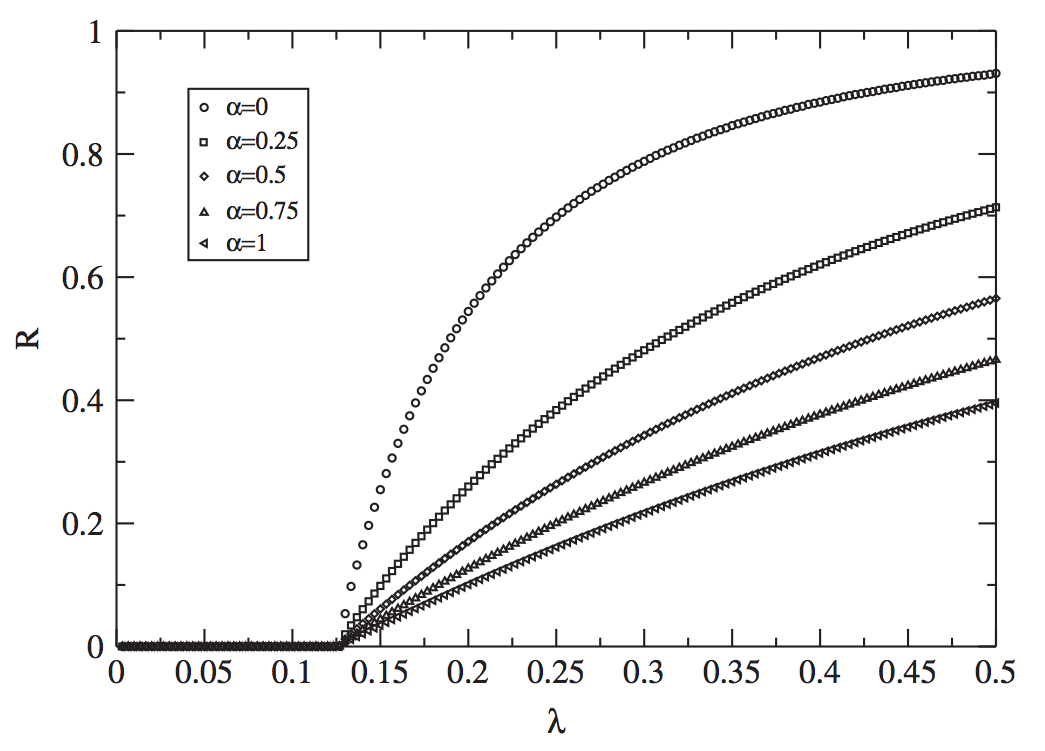
\includegraphics[scale=0.3]{./images/rumor-size-ER}
\end{center}
\caption{Tamanho final do rumor para rede ER, aqui $R$ \'e fun\c{c}\~ao da taxa de espalhamente $\lambda$. A rede considerada tem tamanho $10^6$.}
\label{fig:rumor-size-ER}
\end{figure}


Para a rede ER, o tamanho do rumor exibe uma transi\c{c}\~ao de fase para um certo valor de $\lambda_c$ estimado em 0.12507. Esse resultado parece ser independente de $\alpha$. Nas vizinhan\c{c}as do ponto cr\'itico $R$ se comporta na forma (veja \ref{fig:critical-ER}):

\begin{equation}
R=A(\lambda-\lambda_c)
\label{eq:critical-size-ER}
\end{equation}

\begin{figure}[ht!]
\begin{center}
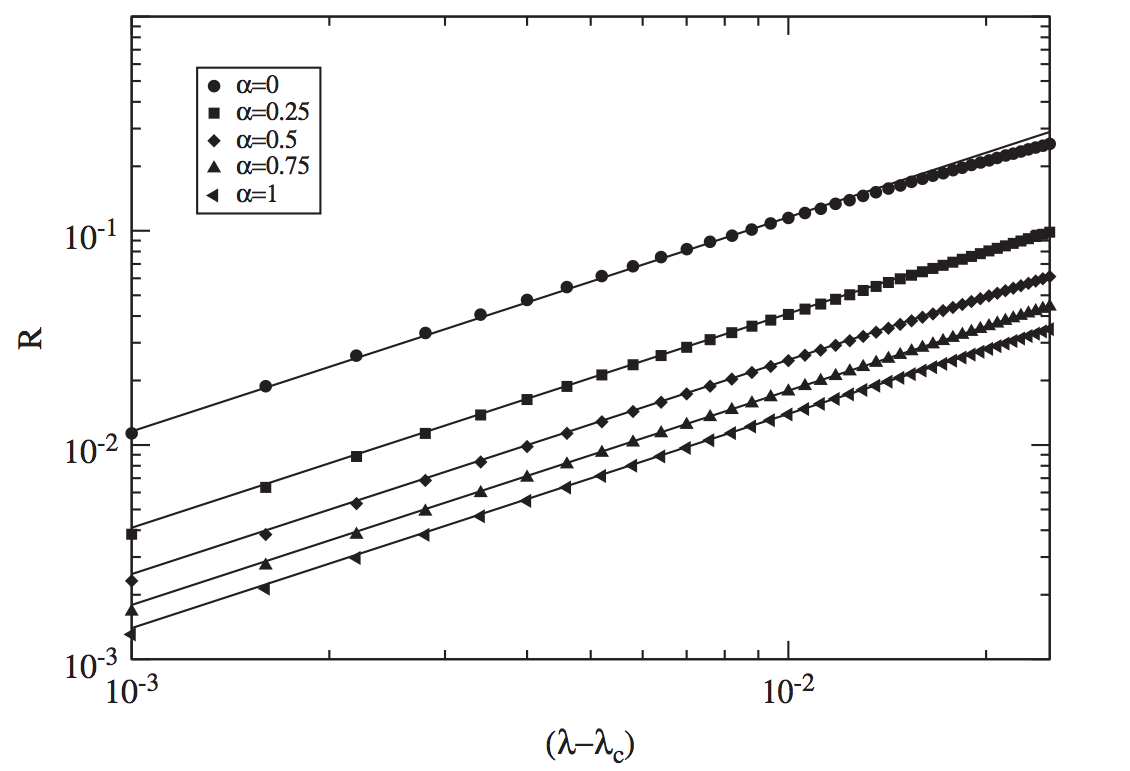
\includegraphics[scale=0.3]{./images/critical-ER}
\end{center}
\caption{Ajuste da equa\c{c}\~ao \ref{eq:critical-size-ER}.}
\label{fig:critical-ER}
\end{figure}


Os resultados para a rede livre de escala s\~ao mostrados na figura \ref{fig:rumor-size-SF}. Outra vez temos um valor limite de $\lambda$ para o qual ocorre epidemia. Note no entanto que esse valor \'e bem menor que para a rede ER. Como o valor de $\lambda_c$ n\~ao depende de $\alpha$ podemos usar o resultado que encontramos para o modelo SIR. As equa\c{c}\~oes para DK com esquecimento se reduzem as do modelo SIR no caso em que $\alpha=0$. Da\'i, conclu\'imos que no limite de uma rede infinita, o valor do limiar tende a zero. 
\begin{figure}[ht!]
\begin{center}
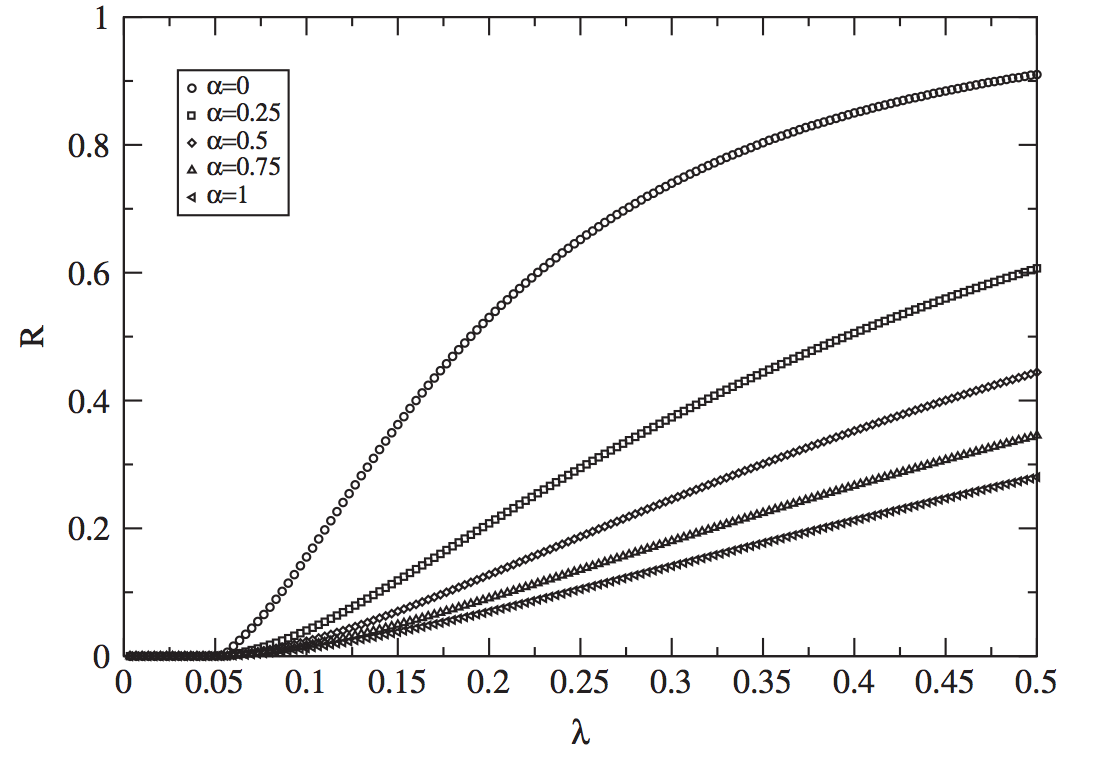
\includegraphics[scale=0.3]{./images/rumor-size-SF}
\end{center}
\caption{Tamanho final do rumor para rede SF com tamanho $N=10^6$.}
\label{fig:rumor-size-SF}
\end{figure}

Para caracterizar ainda mais o comportamento nessa rede, pode-se fitar os resultados com uma exponencial (figura (\ref{fig:critical-SF})):

\begin{equation}
R\sim \exp(-C/\lambda)
\label{eq:critical-size-SF}
\end{equation}
onde o fator $C$ depende varia pouco com $\alpha$. 


\begin{figure}[ht!]
\begin{center}
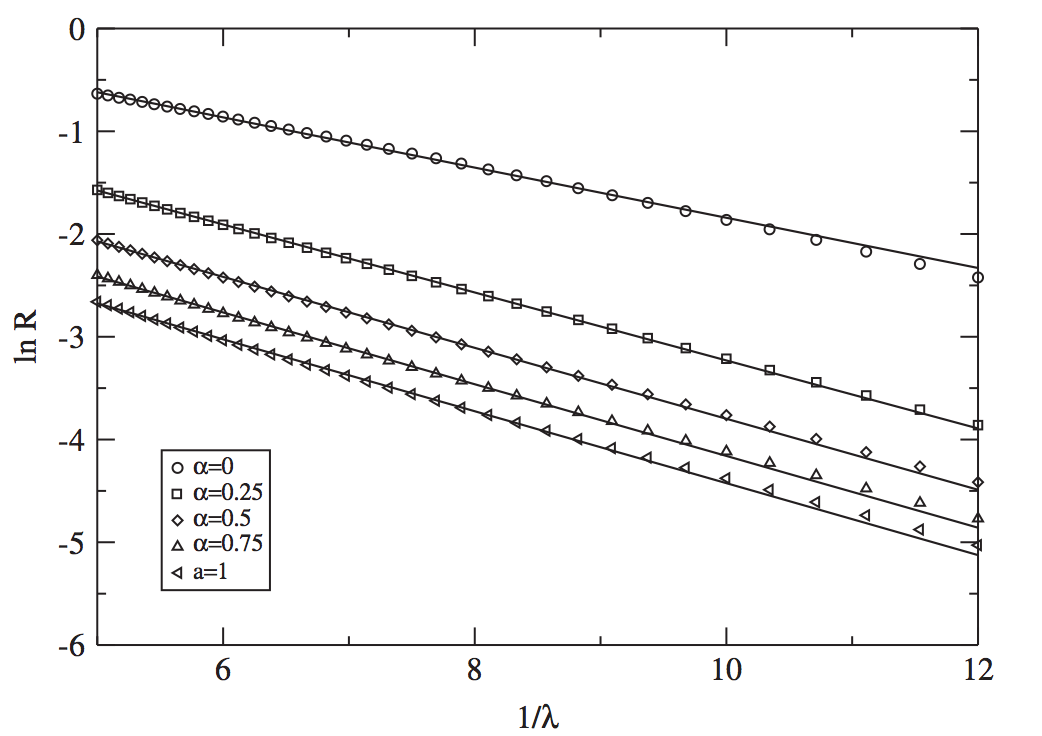
\includegraphics[scale=0.3]{./images/critical-SF}
\end{center}
\caption{Ajuste da equa\c{c}\~ao \ref{eq:critical-size-SF}.}
\label{fig:critical-SF}
\end{figure}

Usando a simula\c{c}\~ao num\'erica tamb\'em pode-se obter a evolu\c{c}\~ao temporal do tamanho do rumor, ilustrado na figura \ref{fig:evol-size-rumor}.


\begin{figure}[ht!]
\begin{center}
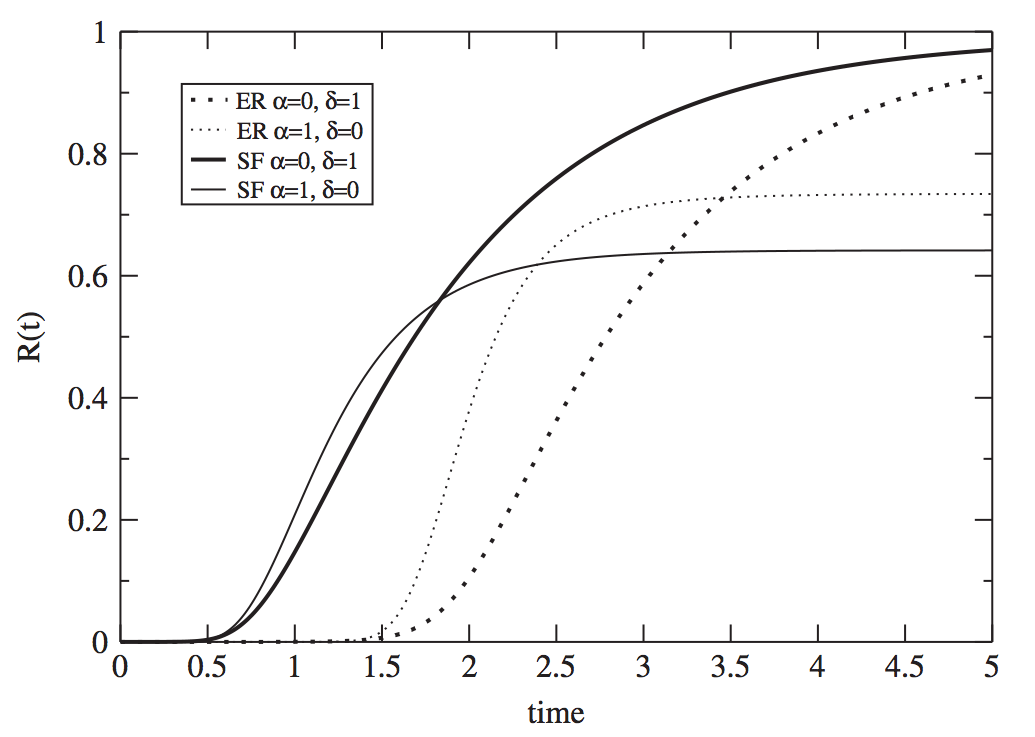
\includegraphics[scale=0.3]{./images/evol-size-rumor}
\end{center}
\caption{Evolu\c{c}\~ao temporal da densidade de indiv\'iduos contidos para as redes consideradas no texto.}
\label{fig:evol-size-rumor}
\end{figure}

%
%\section{rumores}
%-Individuos atingidos por rumores ou noticias <> analogo infecao doencas
%(informados = infectados, porem: um eh intencional o outro involuntario, 
%vantagem vs desvantagem) 
%
%-as perguntas sao similares (numero de atingidos?, limiar de epidemia?, 
%fracao finita vs entorno local), eg: viral strategies in marketting
%
%- os objetivos sao opostos
%
%
%- descrever em epidemias, inventar em informacoes
%
%- interacao assimetrica
%- fluxo unidireccional: vai de quem tem a info, doenca --> para quem nao tem 
%
%-varios dos modelos supoem um limiar na fracao do numero de vizinhos "ativos"
%porem em alguns casos um unico vizinho eh suficiente para iniciar o spreading
%
%- Modelo standard DK (Daley Kendall) 
%ignorants, spreaders, stifflers = S I R
%
%I--> R
%  k
%  k(I+R)
%
%\section{Resultados pr\'evios}
%
%
%rumores: NO THRESHOLD FOR HOMOGENEOUS MIXING (for any rate a finite fraction will 
%be informed)\cite{Castellano:2009ce}
%
%Random, WS tem limiar epidemico, there is an epidemic transition \cite{Zanette:2001kh} 
%correlacoes mudam o limiar
%scale free NAO tem, epidemic threshold ou seja sempre tem epidemia
%
%REDES em evolucao 
%contact switching--> avoids spreading \cite{RisauGusman:2009jh}

%-----------------------------------------------------
% Chapter: Propostas e Conclus\~oes
%-----------------------------------------------------
\chapter{Propostas e Conclus\~oes}
\label{chap:conc}

- outros detalhes em modelos ja estudados
alem das propriedades estacionarias, eh importante caracterizar 
os transientes, quando leva em chegar no SS 

- novos

- difusao

- rumores --> generalizacoes


%%%%%%%%%%%%%%%%%%%%%%%%%%%%
% BIBLIOGRAPHY
%\newpage
\clearpage
\phantomsection
\addcontentsline{toc}{chapter}{Refer\^encias Bibliogr\'aficas}
\bibliography{bib}
\bibliographystyle{unsrt}
%%%%%%%%%%%%%%%%%%%%%%%%%%%%


%%%%%%%%%%%%%%%%%%%%%%%%%%%%
% START APPENDICES
% \appendix
%%%%%%%%%%%%%%%%%%%%%%%%%%%%


%-----------------------------------------------------
% Appendix: Code
%-----------------------------------------------------
%\chapter{Code}
%\label{app:code}

%Este phantom resolve o problema de que a Bibliografia n\~ao aparece no TOC
\phantom{x}

%\begin{verbatim}
%10 PRINT "HELLO WORLD"
%\end{verbatim}


%%%%%%%%%%%%%%%%%%%%%%%%%%%%
% END DOCUMENT
\end{document}
%%%%%%%%%%%%%%%%%%%%%%%%%%%%